\documentclass[10pt,twocolumn,letterpaper]{article}
\usepackage[T1]{fontenc}
\usepackage[utf8]{inputenc}
\usepackage{mathptmx}
\usepackage[left=0.62in,right=0.62in,top=0.72in,bottom=0.78in,columnsep=0.22in]{geometry}
\usepackage{amsmath,amssymb,amsthm}
\usepackage{booktabs,array,multirow,graphicx,xcolor,url,lettrine,balance}
\hyphenation{Para-Ex-press Para-Twin fulfill-ment mar-ket-place con-sign-ment}
\usepackage[hidelinks]{hyperref}
\graphicspath{{figures/}{tex/figures/}}
\usepackage[font=footnotesize,labelsep=period,justification=raggedright,singlelinecheck=false]{caption}
\usepackage{titlesec}
\usepackage{fancyhdr}

% ---- IEEE-like sectioning ----
\renewcommand{\thesection}{\Roman{section}}
\renewcommand{\thesubsection}{\Alph{subsection}}
\titleformat{\section}[block]{\centering\normalsize\scshape}{\thesection.}{0.6em}{}
\titleformat{\subsection}[block]{\normalsize\itshape}{\thesubsection.}{0.5em}{}
\titleformat{\subsubsection}[runin]{\normalsize\itshape}{}{0em}{}[:]
\titlespacing*{\section}{0pt}{9pt plus 2pt}{5pt}
\titlespacing*{\subsection}{0pt}{7pt plus 1pt}{3pt}
\setlength{\parindent}{1em}
\setlength{\abovedisplayskip}{4pt}\setlength{\belowdisplayskip}{4pt}

\newcommand{\IEEEPARstart}[2]{\lettrine[lines=2,findent=2pt,nindent=0pt]{\textbf{#1}}{#2}}
\newenvironment{IEEEkeywords}{\vspace{2pt}\noindent\footnotesize\textit{Index Terms}---}{\vspace{4pt}}
\newcommand{\appendices}{\par\setcounter{section}{0}\setcounter{subsection}{0}%
  \renewcommand{\thesection}{\Alph{section}}%
  \renewcommand{\thesubsection}{\thesection-\Alph{subsection}}%
  \titleformat{\section}[block]{\centering\normalsize\scshape}{Appendix~\thesection}{0.6em}{}}

\pagestyle{fancy}\fancyhf{}
\fancyhead[L]{\scriptsize\scshape PARATECH PLATFORM R\&D TECHNICAL REPORT, VOL. 1, NO. 2, AUGUST 2026 (REVISION 5)}
\fancyhead[R]{\scriptsize\thepage}
\renewcommand{\headrulewidth}{0pt}
\fancypagestyle{plain}{\fancyhf{}\fancyhead[L]{\scriptsize\scshape PARATECH PLATFORM R\&D TECHNICAL REPORT, VOL. 1, NO. 2, AUGUST 2026 (REVISION 5)}\fancyhead[R]{\scriptsize\thepage}\renewcommand{\headrulewidth}{0pt}}

\newtheorem{theorem}{Theorem}
\newtheorem{proposition}{Proposition}
\newtheorem{lemma}{Lemma}
\newtheorem{corollary}{Corollary}
\theoremstyle{definition}
\newtheorem{definition}{Definition}
\newtheorem{assumption}{Assumption}
\newtheorem{remark}{Remark}

\definecolor{openred}{RGB}{150,20,20}
\definecolor{gr}{RGB}{90,90,90}
\newcommand{\OPEN}[3]{{\color{openred}\footnotesize\textsf{[OPEN --- #1 --- owner: #2 --- needed by: #3]}}}
\newcommand{\prov}[1]{{\color{gr}\scriptsize\textsf{[#1]}}}

\begin{document}

\twocolumn[
\begin{@twocolumnfalse}
\vspace*{-8pt}
\begin{center}
{\LARGE ParaExpress: A Mathematically Grounded Hyperlocal\\[2pt]
Fulfillment Network and Digital Twin Architecture\\[2pt]
for Instant Beauty Commerce in Indonesia\par}
\vspace{6pt}
{\large\textsc{Revision 5}\par}
\vspace{8pt}
{\normalsize ParaTech Platform R\&D Team, ParagonCorp\par}
\vspace{10pt}
\end{center}
\begin{quotation}\noindent\footnotesize
\textbf{\textit{Abstract}}---Instant-delivery platforms such as Shopee Express (SPX Instant) and Astro now deliver consumer goods within one hour of order placement, and platforms that own the fastest delivery promise increasingly own the consumer relationship---and, eventually, private-label categories that compete with brand manufacturers. This report specifies \emph{ParaExpress}, a brand-owned hyperlocal fulfillment network and digital twin that allows ParagonCorp, Indonesia's largest beauty company (16 brands, ${\approx}2{,}000$ SKUs and bundles), to fulfill marketplace and direct orders from the fulfillment node nearest the consumer within a sub-60-minute service-level agreement (SLA), while preserving the economics of a manufacturer rather than a platform. We (i) benchmark the fulfillment architectures of Amazon, Alibaba/Cainiao, JD Logistics, Coupang, and quick-commerce operators; (ii) formalize the ParaExpress design problem as an SLA-constrained facility-location, inventory-positioning, and order-routing program, and prove structural results---NP-hardness, a $(1-1/e)$ greedy coverage guarantee \emph{stated within its uncapacitated scope}, unimodality of the network cost in node count yielding a unique optimal micro-fulfillment-center (MFC) count \emph{under a correlation-corrected pooling law}, exact greedy optimality for SKU forward-placement under a uniform matroid, and polynomial-time integrality of real-time order routing; (iii) derive the MFC operating model from these results; (iv) specify new capabilities for the existing MagPie, Heron, Exagon, and ShipGo systems plus three new platform services---a Virtual Inventory \& Distributed Order Management service, an Order Routing Engine, and the ParaTwin digital twin; and (v) define the digital twin's formal state model, data contracts, and experiment portfolio.

Revision~5 corrects five results whose stated scope did not match their use, adds three results the design required and did not have---an order-level fill-rate law, a distribution-free service-radius bound, and a correlation-corrected pooling law---replaces the acceptance gate that could be passed by an incorrect model, adds the gates Phases~3 and~4 lacked, adds the demand-side experiment and the kill criteria the program lacked, and registers twenty-five open items that must be closed before the corresponding decision is taken. The net effect of the corrections is to raise the required node count per metro and to raise the per-SKU availability target; both changes increase the capital ask and neither was visible in Revision~4.
\end{quotation}
\begin{quotation}\noindent\footnotesize
\textit{Index Terms}---Distribution network design, e-commerce fulfillment, facility location, digital twin, last-mile logistics, micro-fulfillment center, order management, quick commerce, supply chain optimization, vehicle routing, order fill rate, risk pooling.
\end{quotation}
\vspace{10pt}
\end{@twocolumnfalse}
]

\renewcommand{\thefootnote}{\fnsymbol{footnote}}
\footnotetext[1]{Manuscript revised August 2026. Supersedes Revision 4 (August 2026). The authors are with the ParaTech Platform Research \& Development Division, PT Paragon Technology and Innovation (ParagonCorp), Jakarta, Indonesia (e-mail: paratech-rnd@paracorpgroup.com). This revision incorporates a structured six-lens design review of Revision~4. Appendix~A documents the review method, the derivation of each correction, and the mapping from finding to change. Open items carried by this revision are registered in Section~XI and marked inline in red.}
\renewcommand{\thefootnote}{\arabic{footnote}}






\section{Introduction}

\IEEEPARstart{T}{he} economics of consumer commerce in Southeast Asia are being reorganized around the \emph{delivery promise}. Shopee's in-house carrier SPX Express advertises same-day and instant fulfillment in Indonesian metros; quick-commerce operator Astro operates a dense network of dark stores that put a courier at the consumer's door in as little as 15--60 minutes. International precedents---Amazon's regionalized same-day and Freshippo store-warehouses, JD Logistics' integrated fulfillment estate, and Coupang's density-first Rocket Delivery---demonstrate a consistent endgame: \emph{whoever controls the fastest fulfillment loop accumulates the consumer relationship, the data, and ultimately the shelf}, including private-label brands that displace incumbent manufacturers.

ParagonCorp is Indonesia's largest beauty manufacturer, operating 16 brands (Wardah, Make Over, Emina, Kahf, Instaperfect, Crystallure, Labor\'e, Biodef, Tavi, Wonderly, Beyondly, OMG, Earth Love Life, Putri, and others) across roughly 2,000 active SKUs and bundles. Its current distribution stack---a National Distribution Centre (NDC) in Jakarta, a B2C DC in Tegal serving TikTok Shop and Shopee order flow, and a set of B2B DCs (Bogor, Bandung, Solo, Makassar, and others, including Malaysia) serving general- and modern-trade stores---was engineered for \emph{replenishment logistics}: moving cases to stores and parcels within days. It was not engineered for \emph{instant logistics}: moving a single eyeliner to a consumer in under an hour.

This asymmetry is now strategic. If marketplaces alone can meet the instant promise, ParagonCorp's brands become undifferentiated supply behind someone else's delivery experience. The competitive response specified here is not to out-build Shopee's parcel network, but to \emph{redefine the fulfillment layer for the beauty category}: a hyperlocal, brand-owned network of micro-fulfillment centers (MFCs) and consignment-store fulfillment nodes, fed by the existing NDC/DC backbone, replenished via digital mid-mile partners, and delivering through established on-demand fleets---so that \emph{any} channel order is fulfilled by the nearest ParagonCorp-controlled node, faster and cheaper per beauty basket than a generalist dark store can achieve.

\subsection{What Revision 5 Changes}

Revision~4 of this report was subjected to a structured six-lens design review before release. The review produced forty-eight candidate findings. Seven were discarded in an adversarial pass (Appendix~A-E). Of the forty-one that survived, thirteen required new or restated mathematics, fourteen required specification changes, and fourteen could not be resolved without facts nobody has confirmed and are registered as open items in Section~\ref{sec:open}, where they expand into twenty-five register rows because several name more than one quantity. Appendix~A gives the review method, the finding register, and the derivation of every correction with its supporting literature. The material changes are:

\begin{enumerate}
\item \textbf{The availability promise was arithmetically unreachable as specified.} Revision~4 set inventory targets from a per-SKU fill rate and promised 95\% attainment at the \emph{order} level. Because a PX1 order fails if any SKU in its basket is unavailable, the two are different quantities. Proposition~\ref{prop:orderfill} gives the inversion. Under an illustrative basket-size distribution with mean 2.45 distinct SKUs, a 98\% per-SKU target yields 95.2\% order availability before any queueing, picking, or travel variability is counted; at mean 3.05 SKUs it yields 94.0\%, below the promise.
\item \textbf{The service radius was computed from a quantile identity that does not hold.} Revision~4's Proposition~2 subtracted a single $\alpha$-quantile of in-node time from the promise budget and treated travel as deterministic at a mean speed. The PX1 constraint requires the $\alpha$-quantile of a \emph{sum}, and quantiles are not additive \cite{artzner1999,embrechts2002}. Proposition~\ref{prop:radius} gives a distribution-free replacement via an explicit risk-budget split. On illustrative parameters the feasible radius falls from 13.3\,km to 7.1\,km, raising the SLA node floor by a factor of $3.5$; whether that floor binds depends on parameters that are not yet measured.
\item \textbf{The risk-pooling penalty assumed a demand independence the design itself breaks.} Revision~4's Proposition~1 used the $\sqrt{n}$ safety-stock law, which holds only for independent zone demand. The design models live-commerce demand as spatially correlated Hawkes bursts and gives the distributed order manager cross-node substitution and rebalancing. Proposition~\ref{prop:pooling} restates the penalty under equicorrelated demand; Eppen's original result already covers this case \cite{eppen1979}. Theorem~\ref{thm:nodecount} is restated on the corrected law. On the illustrative parameters of Revision~4, moving from $\rho=0$ to $\rho=0.3$ raises the optimal node count from 9.1 to 13.2.
\item \textbf{Two theorems were cited outside their proven scope.} The $(1-1/e)$ coverage guarantee is proved for the uncapacitated case and was used to order a rollout in a network with hard node throughput caps; the real-time routing optimality result is proved for one wave and was used to justify continuous re-solving. Both scopes are now stated explicitly, and Section~\ref{sec:structural}-\ref{sec:capacitated} states what is and is not known for the capacitated variant.
\item \textbf{The oversell guarantee did not cover the operations the system performs.} Proposition~4 of Revision~4 assumed a single ledger partition; the distributed order manager rebalances stock \emph{across} partitions, and the store client may run offline for hours. Proposition~\ref{prop:atp} restates the invariant with a cross-partition commit rule and an effective-latency definition that accounts for the offline window.
\item \textbf{Staffing assumed Poisson arrivals into a wave-batched system.} Proposition~\ref{prop:staffing} restates square-root staffing under compound-Poisson (wave) arrivals. The inflation factor is $\sqrt{1+\lambda_f\Delta}$, which makes the wave length $\Delta$ an explicit trade between routing optimality and picker headcount.
\item \textbf{An acceptance gate tested model agreement rather than reality, two phases had no gate at all, and the program had no stop condition.} Section~\ref{sec:roadmap} re-cuts the Phase~1 gate against the design target, adds gates to Phases~3 and~4, adds a demand-side experiment (E7) and an incrementality holdout (E8), and states explicit kill criteria.
\item \textbf{Facts nobody has confirmed are no longer written as facts.} Twenty-five open items are tagged inline and registered in Section~\ref{sec:open}. Ten of them block Phase~0: eight must close before Phase~0 exits, and two before it starts.
\end{enumerate}

The contributions of this report are: (1) a state-of-the-art benchmark of global and regional instant-fulfillment architectures (Section~\ref{sec:bench}); (2) a formal mathematical definition of the ParaExpress network design problem, with theorems and propositions that justify the architecture and make it computable (Sections~\ref{sec:formal}--\ref{sec:structural}); (3) the ParaExpress reference network architecture and MFC operating model derived from those results (Sections~\ref{sec:arch}--\ref{sec:mfc}); (4) the business model and partnership topology (Section~\ref{sec:business}); (5) the solution specification (Section~\ref{sec:solution}); (6) the ParaTwin formal model, data contracts, and experiment plan (Section~\ref{sec:twin}); (7) a phased implementation roadmap with pilot acceptance criteria and kill criteria (Section~\ref{sec:roadmap}); and (8) an open-items register (Section~\ref{sec:open}) and a review-method appendix (Appendix~A).

\section{State-of-the-Art Benchmark}\label{sec:bench}

We benchmark the fulfillment architectures that define the global and regional state of the art, then extract the design lessons that ParaExpress adopts or deliberately inverts. Table~\ref{tab:bench} summarizes.

\emph{Provenance convention.} Revision~4 grouped citations per row, which allowed a press-derived estimate and a disclosed operating figure to sit in the same table without distinction. Every cell in Table~\ref{tab:bench} now carries a mark: $\dagger$ for a figure disclosed by the operator or its regulator filings, $\ddagger$ for a figure reported by trade press or a third party and not confirmed by the operator, and $\star$ for a ParaExpress design target rather than an observation.

\subsection{Amazon: Regionalization and Sub-Same-Day Sites}
Amazon's United States network is a multi-echelon hierarchy of inbound cross-docks, fulfillment centers (FCs), sortation centers, and delivery stations---more than 600 logistics sites \cite{redstag}. Two recent moves matter most for ParaExpress. First, the 2023 \emph{regionalization} partitioned the national network into eight largely self-sufficient regions, with fast-moving inventory replicated in each; in-region fulfillment rose from 62\% to 76\% of ordered products, and 2023 cost-to-serve fell by more than \$0.45 per unit---the first reduction since 2018---while over 7 billion items were delivered same- or next-day \cite{chandra2026,amazonscience,supplychaindive2023}. Second, Amazon's \emph{sub-same-day} (SSD) sites---facilities roughly one-tenth the size of a classical FC that collapse FC, sortation, and delivery station under one roof---achieve an average pick-to-outbound-dock time of 11 minutes and anchor the same-day promise in the top metros, where about 60\% of Prime orders now arrive same- or next-day \cite{costar2024,palmer2024}. Amazon's anticipatory-shipping patent formalizes the underlying doctrine: move inventory toward predicted demand \emph{before} the order exists \cite{spiegel2013}. Robotics (the million-robot fleet, Sequoia stowing) compresses in-node time \cite{amazon2023robots,techcrunch2025}.

\subsection{Alibaba/Cainiao and the Freshippo Store-as-Warehouse}
Cainiao orchestrates a largely partner-operated network (${\sim}170$--200 warehouses, 170,000+ neighborhood pickup points) through a data layer---the standardized electronic waybill---rather than through asset ownership, and offers half-day/same-day products in ${\sim}300$ cities \cite{wirechina2024,scmp2023}. The most transferable pattern for ParagonCorp is Freshippo (Hema): each store doubles as a fulfillment node with in-aisle picking, overhead-conveyor consolidation, and a 30-minute promise within a 3\,km radius; about 60\% of store throughput is online orders \cite{vangaalen2022}. Freshippo proves that \emph{existing retail assets can be converted into an instant-fulfillment network} when picking and inventory accuracy are engineered deliberately---precisely the ParaExpress consignment-store thesis. It is also the closest analogue to the partner-compliance problem registered as open items O-5 and O-14.

\subsection{JD Logistics: Front Distribution Centers}
JD holds first-party inventory deep in the network---800+ warehouses organized as 8 large regional distribution centers (RDCs) feeding small, district-level \emph{front distribution centers} (FDCs) stocked with local fast movers---and delivers ${\sim}90\%$ of orders same- or next-day \cite{statista2024}. JD's deployed assortment-planning and inventory-allocation system (forecasting + optimization + simulation over all eight RDCs) reports savings of \$6.1M/yr in holding cost and \$22.3M/yr in transfer cost with a $+0.85$ pp availability gain \cite{wang2025}---direct evidence that the forward-assortment problem (P2) and its digital-twin evaluation loop are where the money is.

\subsection{Coupang: Density as Strategy}
Coupang's Rocket Delivery guarantees next-day (and dawn) delivery on millions of SKUs; the structural fact is density---70\% of South Koreans live within ${\sim}11$\,km of a Coupang fulfillment center, across 100+ facilities and 55M+ sq ft built with ${\sim}\$4.6$B of cumulative logistics investment \cite{goodwater2021,coupang2025}. Coupang demonstrates the endgame ParagonCorp must respect: once a platform achieves fulfillment density, it converts speed into membership lock-in.

\subsection{Quick Commerce: Failures Abroad, Proof in India}
The 2021--2024 dark-store wave supplies both the template and the cautionary tale. The template: 200--700\,m$^2$ dark stores, 1,000--3,500 SKUs, 1.5--3\,km radius, 10--30-minute promises; delivery-cycle anatomy of 2--3 min pick, ${\sim}1$ min rider assignment, 5--6 min transit \cite{suitefleet2025,storyboard2025}. The cautionary tale: Getir fell from an \$11.8B valuation to a retreat from all Western markets in April 2024, after promotion-fueled growth with sub-scale order density and low AOV \cite{browne2024,sifted2024}. The proof: India's Blinkit (1,800+ dark stores) and Zepto turned the same template contribution-margin positive via order density, AOV discipline, and disciplined assortment \cite{mohan2025,storyboard2025}.

The ParaExpress inference is category-structural: beauty baskets carry 2--4$\times$ grocery AOV, zero cold chain, and high value density, so the same dark-store mechanics should clear break-even at lower order density than grocery. \emph{Revision~5 note:} Revision~4 supported this claim by citation to its own design-target P\&L, which is circular. The claim is now stated as a hypothesis with a named test (experiment E7, Section~\ref{sec:twin}) and a kill criterion (Section~\ref{sec:roadmap}). \OPEN{observed instant-attach rate, conversion lift, and delivery-fee willingness-to-pay for beauty on an Indonesian marketplace}{Commercial Lead}{Phase 0 exit}

\subsection{Store-Based Fulfillment: Walmart and Target}
Walmart reaches 93\% of US households with same-day delivery from ${\sim}3{,}900$ stores; store-fulfilled delivery sales tripled in one year to over \$1B/month \cite{scd2025}. Target fulfills 95\%+ of total orders from stores, using sortation centers and the Shipt fleet for next-day delivery \cite{target2023}. Both raise warehouse pick efficiency for near-zero incremental real estate and radically shorter last miles---the exact trade Corollary~\ref{cor:stores} formalizes for ParagonCorp's consignment estate.

\subsection{The Indonesian Battlefield}
Shopee holds ${\sim}46\%$ of Indonesian e-commerce GMV and a dominant ${\sim}63\%$ share of platform beauty GMV \cite{magpieiq2026,databoks2024}; its carrier SPX Express covers 514 cities/regencies, and in February 2025 Shopee deployed 200 micro-fulfillment centers in tier-2/3 cities (a US\$120M program targeting ${\sim}40\%$ faster delivery) \cite{spx2025,mordor2024}. TikTok Shop/Tokopedia reached ${\sim}$US\$13.8B Indonesian GMV in 2025 \cite{moca2026}, following ByteDance's 2023 acquisition of a controlling stake in Tokopedia \cite{nikkei2023}. Astro operates ${\sim}50$ dark stores in Jabodetabek with ${\sim}1{,}500$ hyperlocalized SKUs, 2--3\,km radii, and 15-minute delivery \cite{theken2023,gpca2024}. On-demand last-mile capacity is commoditized and API-accessible: GrabExpress Instant (pickup ${\sim}30$ min, distance-based per-km pricing) and GoSend Instant (max 40\,km, 20\,kg, lifecycle webhooks) both expose merchant APIs \cite{grab2025,gojek2024}. Mid-mile digital 3PL capacity exists in MOSTRANS (Kalbe/Enseval group): 70+ transporters, 5,000+ GPS-equipped trucks, ambient/cool/cold chain, e-POD, and ERP integration \cite{ssi2022,kalbe2019}. Indonesian quick commerce is projected to grow from ${\sim}$US\$1.4--3.1B (2025, definitions vary) at 6--8\% CAGR, with minimarket chains (Alfamart ${\sim}50$ dark stores) entering O2O fulfillment \cite{rm2026}---evidence that the instant tier is becoming table stakes, not a niche.

\emph{The competitive fact this revision makes explicit:} Shopee is simultaneously the largest demand channel for ParagonCorp beauty and a direct operator in the fulfillment layer ParaExpress proposes to occupy. The entire PX1 promise on marketplace channels depends on Shopee and TikTok Shop permitting seller-fulfilled instant orders from ParagonCorp's own nodes. Revision~4 asserted this permission. It is now open item~O-1 and a Phase~0 exit gate. \OPEN{written confirmation from at least one marketplace that seller-fulfilled instant from brand-operated nodes is permitted, and on what courier terms}{Commercial Lead}{Phase 0 exit}

\subsection{Design Lessons Adopted by ParaExpress}
\textbf{L1. Regionalize inventory ahead of demand}; measure in-region fulfillment share as a first-class KPI (Amazon) \cite{chandra2026}.
\textbf{L2. Collapse echelons for speed}: the instant tier needs single-roof pick-to-courier in $\leq 11$--15 min, not a chain of touches (Amazon SSD, Blinkit) \cite{costar2024,storyboard2025}.
\textbf{L3. Convert existing retail into fulfillment}: engineered in-store picking with a hard promise radius (Freshippo, Walmart, Target) \cite{vangaalen2022,scd2025,target2023}.
\textbf{L4. Solve assortment + allocation with a simulation loop}, not spreadsheets (JD) \cite{wang2025}.
\textbf{L5. Density before geography}: saturate one metro to SLA-profitability before replicating (Coupang; Getir's inverse) \cite{goodwater2021,browne2024}.
\textbf{L6. Respect unit economics}: AOV discipline and order density decide survival (India QC) \cite{mohan2025}.
\textbf{L7. Own the data plane, rent the assets}: electronic-waybill-style standardization over partner fleets (Cainiao; MOSTRANS/Grab for ParagonCorp) \cite{wirechina2024,grab2025}.
\textbf{L8. The promise is computed, not configured}: dynamic, honest delivery promises shown pre-checkout drive conversion (all benchmarks).
\textbf{L9 (new in Revision 5). A promise is only as honest as the staleness of its inputs.} A computed promise served from a cache is a configured promise with extra steps unless the cache's staleness is bounded per input and the fastest-moving input sets the refresh rate. This lesson is implemented in Section~\ref{sec:solution} as an explicit per-input staleness contract on the Available-to-Deliver (ADR) API.

\section{Formal Problem Definition}\label{sec:formal}

We give a formal definition of the ParaExpress design problem. The formulation is deliberately layered: a \emph{strategic} layer (where to open fulfillment nodes and what to stock), a \emph{tactical} layer (replenishment and staffing), and an \emph{operational} layer (real-time order routing and dispatch). Each layer is an optimization problem whose structure we exploit in Section~\ref{sec:structural}, and each is mirrored one-to-one by a module of the ParaTwin digital twin (Section~\ref{sec:twin}).

\subsection{Network, Demand, and SLA Primitives}

\begin{definition}[Fulfillment graph]
The ParaExpress network is a directed graph $G=(\mathcal{N},\mathcal{A})$ whose node set $\mathcal{N}=\{0\}\cup\mathcal{D}\cup\mathcal{F}\cup\mathcal{Z}$ comprises the NDC (node 0), the set of regional DCs $\mathcal{D}$ (B2C DC Tegal and B2B DCs), the set of candidate fulfillment nodes $\mathcal{F}=\mathcal{F}^{\mathrm{mfc}}\cup\mathcal{F}^{\mathrm{store}}$ (own micro-fulfillment centers and Exagon consignment stores), and the set of demand zones $\mathcal{Z}$ (e.g., kelurahan-level polygons). Arcs $\mathcal{A}$ carry mid-mile flows ($0\to\mathcal{D}\to\mathcal{F}$) and last-mile flows ($\mathcal{F}\to\mathcal{Z}$).
\end{definition}

\begin{definition}[Demand field]
Let $\mathcal{K}$ denote the SKU catalog, $|\mathcal{K}|\approx 2{,}000$ across 16 brands. Instant-channel demand in zone $z\in\mathcal{Z}$ for SKU $k\in\mathcal{K}$ is a marked Poisson process with rate $\lambda_{zk}\ge 0$ orders per hour; $\lambda_z=\sum_k\lambda_{zk}$ and $\Lambda=\sum_z\lambda_z$. Order composition (basket of SKUs and bundle explosions) follows a distribution $\mathcal{B}_z$ estimated from MagPie history. We write $p_j=\Pr[\,|B|=j\,]$ for the distribution of the number of \emph{distinct} SKUs in a basket, and $G_B(x)=\sum_{j\ge 1}p_jx^{j}$ for its probability generating function. \OPEN{empirical $p_j$ and $G_B$ from MagPie B2C order history, by metro and by channel}{Data Lead}{Phase 0 exit}
\end{definition}

\begin{definition}[Service promise]
A promise class is a pair $(\tau,\alpha)$: the order must be delivered within $\tau$ minutes of payment with probability at least $\alpha$. ParaExpress operates three classes: $\mathrm{PX1}=(60\,\mathrm{min},0.95)$ (instant), $\mathrm{PX2}=(240\,\mathrm{min},0.95)$ (same-day slot), and $\mathrm{PX3}$ (next-day, fulfilled by the existing Tegal B2C DC flow). The end-to-end sojourn of an order decomposes as
\begin{equation}\label{eq:sojourn}
T=T_{\mathrm{route}}+T_{\mathrm{queue}}+T_{\mathrm{pick}}+T_{\mathrm{handover}}+T_{\mathrm{travel}},
\end{equation}
i.e., routing decision, waiting for a picker, pick+pack, courier pickup, and travel to the consumer. We write $T_{\mathrm{node}}=T_{\mathrm{queue}}+T_{\mathrm{pick}}+T_{\mathrm{handover}}$ throughout, and reserve $T_{\mathrm{travel}}$ for the stochastic last-mile leg. \emph{Revision~5 note:} Revision~4 used the symbol $t^{\alpha}_{\mathrm{node}}$ in a way that silently required $T_{\mathrm{travel}}$ to be deterministic; see Proposition~\ref{prop:radius}.
\end{definition}

\begin{definition}[Availability]\label{def:avail}
Two distinct availability quantities are used in this report and must not be interchanged. The \emph{item fill rate} $\beta$ is the probability that a given SKU is on hand at a node when requested. The \emph{order fill rate} $\alpha_B$ is the probability that \emph{every} SKU in a basket is on hand at the assigned node. Revision~4 set inventory targets from $\beta$ and stated the promise in terms of $\alpha_B$ without an inversion between them; Proposition~\ref{prop:orderfill} supplies it.
\end{definition}

\subsection{Strategic Layer: SLA-Constrained Location--Allocation}

Binary variables $y_f\in\{0,1\}$ open node $f\in\mathcal{F}$ (for a consignment store, ``opening'' means activating it as a fulfillment node with dedicated ParaExpress stock and app tooling); $x_{fz}\in[0,1]$ is the fraction of zone $z$'s instant demand assigned to $f$. Let $t_{fz}$ be the $\alpha$-quantile of $T$ in \eqref{eq:sojourn} when $f$ serves $z$ (travel time from the road network / Grab historical data), and let the \emph{coverage set} be $\mathcal{F}(z)=\{f: t_{fz}\le\tau\}$. With fixed cost $c^{\mathrm{fix}}_f$ per period (rent, staff, equipment amortization; near-zero for store nodes), variable fulfillment cost $c^{\mathrm{var}}_{fz}$ per order (pick, pack, courier fee $f\to z$), and per-order gross margin $m$, the strategic problem is:
\begin{align}
(\mathrm{P1})\quad \max_{x,y}\ &\sum_{z\in\mathcal{Z}}\sum_{f\in\mathcal{F}(z)}\bigl(m-c^{\mathrm{var}}_{fz}\bigr)\lambda_z x_{fz}-\sum_{f\in\mathcal{F}}c^{\mathrm{fix}}_f y_f \label{eq:p1}\\
\text{s.t.}\ &\textstyle\sum_{f\in\mathcal{F}(z)}x_{fz}\le 1,\quad \forall z\in\mathcal{Z},\label{eq:p1a}\\
&x_{fz}\le y_f,\quad \forall f,z,\label{eq:p1b}\\
&\textstyle\sum_z\lambda_zx_{fz}\le\mu_fy_f,\quad\forall f\in\mathcal{F},\label{eq:p1c}\\
&x_{fz}\ge 0,\ y_f\in\{0,1\},\nonumber
\end{align}
where $\mu_f$ is node $f$'s sustainable throughput (orders/hour) from its staffing and layout (Section~\ref{sec:mfc}). Constraint \eqref{eq:p1a} allows demand to remain unserved by PX1 (it falls back to PX2/PX3), \eqref{eq:p1b} links assignment to opening, and \eqref{eq:p1c} enforces throughput. (P1) generalizes the capacitated facility-location problem \cite{daskin2013,melo2009} with an SLA-induced coverage structure \cite{church1974}.

\subsection{Strategic Layer: Forward Assortment}

An MFC cannot hold 2,000 SKUs; it holds a forward assortment $S_f\subseteq\mathcal{K}$ limited by shelf capacity $V_f$ (slots). Let $w_k$ be the slot requirement of SKU $k$ and $r_{fk}$ the instant-demand revenue rate captured if $k$ is stocked at $f$ (orders containing an unstocked SKU either split, downgrade to PX2, or are lost with probability $\theta$). The assortment problem at node $f$ is
\begin{equation}\label{eq:p2}
(\mathrm{P2})\quad \max_{S\subseteq\mathcal{K}}\ \sum_{k\in S}r_{fk}\quad\text{s.t.}\quad\sum_{k\in S}w_k\le V_f.
\end{equation}
With basket effects the objective generalizes to $R_f(S)=\mathbb{E}_{\mathcal{B}}\bigl[m(B)\,\mathbf{1}\{B\subseteq S\}\bigr]$ over baskets $B$, which is monotone but not modular; Section~\ref{sec:structural} gives exact and approximate solutions for the practically relevant cases.

\subsection{Tactical Layer: Inventory Positioning and Replenishment}

Each stocked SKU $k$ at node $f$ follows a periodic base-stock policy with review period $T_r$ (replenishment wave from the parent DC via mid-mile), lead time $L_f$, and base-stock level
\begin{equation}\label{eq:basestock}
b_{fk}=\underbrace{\lambda_{fk}(T_r+L_f)}_{\text{cycle stock}}+\underbrace{z_{\beta^\star}\,\sigma_{fk}\sqrt{T_r+L_f}}_{\text{safety stock}},
\end{equation}
where $\lambda_{fk},\sigma_{fk}$ are the mean and standard deviation \emph{per unit time} of demand allocated to $f$, $z_{\beta^\star}=\Phi^{-1}(\beta^\star)$, and $\beta^\star$ is the \emph{item} fill rate implied by the \emph{order} fill target through Proposition~\ref{prop:orderfill}. \emph{Revision~5 note:} Revision~4 wrote $z_\beta$ with $\beta$ read directly from the PX1 promise, which is the substitution Proposition~\ref{prop:orderfill} forbids. Replenishment quantities feed a mid-mile vehicle-routing problem over $\mathcal{D}\to\mathcal{F}$ executed by the 3PL (MOSTRANS), a capacitated VRP with time windows \cite{toth2014}. The modern algorithmic landscape for this class is well charted: hybrid genetic search (HGS) with the SWAP* neighborhood is the quality benchmark for the CVRP \cite{vidal2022,wouda2024}; adaptive large neighborhood search (ALNS) is the reference framework for rich pickup-and-delivery variants \cite{ropke2006,voigt2025}; and LKH-3 remains the standard cross-check solver \cite{helsgaun2017}. Section~\ref{sec:solution} specifies which member of this portfolio each ParaExpress routing surface uses.

\subsection{Operational Layer: Real-Time Order Routing}

At decision epoch $t$, let $O(t)$ be the set of open instant orders and for order $o$ let $\mathcal{F}(o)\subseteq\mathcal{F}$ be the nodes that (i) cover $o$'s zone within the promise, (ii) have all SKUs of $o$'s basket in available-to-promise (ATP) virtual inventory, and (iii) have residual picking capacity. With routing cost $c_{of}$ (courier fee + marginal congestion cost + inventory-displacement penalty), the router solves
\begin{align}
(\mathrm{P3})\quad\min_u\ &\sum_{o\in O(t)}\sum_{f\in\mathcal{F}(o)}c_{of}u_{of}\label{eq:p3}\\
\text{s.t.}\ &\textstyle\sum_f u_{of}=1\ \ \forall o,\qquad \sum_o u_{of}\le\kappa_f(t)\ \ \forall f,\nonumber
\end{align}
with $u_{of}\in\{0,1\}$ and $\kappa_f(t)$ the remaining slot capacity of $f$ in the current wave. (P3) is re-solved once per wave by the Order Routing Engine under the commitment policy of Section~\ref{sec:structural}-\ref{sec:commit}; Theorem~\ref{thm:routing} shows it is exactly solvable in real time.

\subsection{Operational Layer: In-Node Queueing and Dispatch}

Node $f$ with $c_f$ pickers is modeled as a queue with wave-batched arrivals at aggregate rate $\lambda_f=\sum_z\lambda_zx_{fz}$ and pick+pack rate $\nu$ per picker. Courier arrival after handover request is an independent delay $D^{\mathrm{grab}}_f$ (empirically log-normal from Grab/GoSend APIs). The PX1 promise requires
\begin{equation}\label{eq:px1}
\Pr\bigl[T_{\mathrm{node}}+T_{\mathrm{travel}}\le\tau-T_{\mathrm{route}}\bigr]\ge\alpha,
\end{equation}
which couples staffing $c_f$, wave length $\Delta$, and service radius to demand (Propositions~\ref{prop:radius} and~\ref{prop:staffing}).

\section{Structural Results}\label{sec:structural}

The formulations above are not merely descriptive; their mathematical structure dictates the ParaExpress architecture. This section states the results and their design consequences. Proofs are given inline when short and sketched otherwise. Results marked $^{\mathrm{R5}}$ are new or materially restated in Revision~5; each carries a note explaining what changed and why.

\subsection{Hardness and Why a Digital Twin Is Necessary}

\begin{theorem}[NP-hardness of network design]\label{thm:hardness}
Problem \eqref{eq:p1} is NP-hard, even with uncapacitated nodes, uniform margins, and a single SKU.
\end{theorem}
\begin{proof}
Take an instance of \textsc{Set Cover} with universe $U$ and family $\mathcal{S}$. Build one demand zone per element $u\in U$ with $\lambda_z=1$ and one candidate node per set $S\in\mathcal{S}$ with $t_{fz}\le\tau$ iff $u\in S$, $c^{\mathrm{fix}}_f=\varepsilon$, $\mu_f=\infty$, and $m-c^{\mathrm{var}}_{fz}=M\gg|\mathcal{S}|\varepsilon$. Any optimal solution of \eqref{eq:p1} covers all zones (each unit of covered demand is worth $M$), and among covering solutions maximizing \eqref{eq:p1} is equivalent to minimizing $\sum_fy_f$; hence an optimal (P1) solution yields a minimum set cover. \textsc{Set Cover} is NP-hard \cite{garey1979}, so (P1) is NP-hard.
\end{proof}

\begin{remark}
Theorem~\ref{thm:hardness} is the formal design justification for the ParaTwin program: the strategic design space cannot be searched exactly at national scale, so ParaExpress pairs (i) approximation algorithms with provable guarantees for candidate generation with (ii) high-fidelity digital twin simulation for candidate evaluation, rather than trusting a single monolithic MILP solve.
\end{remark}

\subsection{Coverage Is Submodular in the Uncapacitated Case}

\begin{theorem}[Near-optimal greedy expansion, uncapacitated]\label{thm:greedy}
Let $g(Y)$ denote the optimal value of \eqref{eq:p1} restricted to open set $Y\subseteq\mathcal{F}$ with the fixed-cost term removed. \textbf{Assume $\mu_f=\infty$ for all $f$.} Then $g$ is monotone nondecreasing and submodular. Consequently, for any budget of $p$ nodes, the greedy algorithm that repeatedly opens the node with the largest marginal covered contribution attains at least $(1-1/e)\approx 63.2\%$ of the optimal covered contribution, and this is the best possible guarantee for any polynomial algorithm unless P${=}$NP.
\end{theorem}
\begin{proof}
With $\mu_f=\infty$, each zone is served entirely by its best open node, so $g(Y)=\sum_z\lambda_z\max_{f\in Y\cap\mathcal{F}(z)}(m-c^{\mathrm{var}}_{fz})^+$ (with $\max_\emptyset=0$). Each summand is a maximum of nonnegative node-values over the chosen set, which is monotone and submodular; nonnegative sums preserve both properties. The $(1-1/e)$ guarantee for greedy maximization of a monotone submodular function under a cardinality constraint is the classical result of Nemhauser, Wolsey and Fisher \cite{nemhauser1978}, applied to a location problem of this form by Cornuejols, Fisher and Nemhauser \cite{cornuejols1977}; the matching inapproximability bound is Feige's \cite{feige1998}.
\end{proof}

\subsubsection*{$^{\mathrm{R5}}$ Scope of Theorem~\ref{thm:greedy} under capacity}\label{sec:capacitated}

Revision~4 stated Theorem~\ref{thm:greedy} for the uncapacitated case and then used it, through Corollary~\ref{cor:stores}, to order a rollout in a network where constraint~\eqref{eq:p1c} binds and Table~\ref{tab:formats} caps node throughput between 20 and 150 orders per hour for the two measured formats, with the store-node cap itself unmeasured (O-14). That is a use outside the proven scope, and the scope matters: under capacity the guarantee does not transfer.

Let $g^{\mathrm{cap}}(Y)$ be the optimal value of \eqref{eq:p1}--\eqref{eq:p1c} over open set $Y$ with fixed costs removed. Three statements hold, and Revision~4 did not distinguish them.

\emph{(a) Monotonicity survives.} Opening a node relaxes \eqref{eq:p1c} and adds columns, so $g^{\mathrm{cap}}$ is nondecreasing. Corollary~\ref{cor:stores}, which uses only monotonicity and $c^{\mathrm{fix}}\approx0$, is therefore unaffected by capacity.

\emph{(b) Submodularity fails for whole-order assignment.} The proof of Theorem~\ref{thm:greedy} works because each zone independently selects its best open node; that argument collapses the moment \eqref{eq:p1c} binds. It does more than collapse. The following instance, found by exhaustive search over small cases, violates diminishing returns outright. Three candidate nodes $\{0,1,2\}$ and three zones with demand rates $\lambda=(0.6,\,1.0,\,0.4)$ and node throughputs $\mu=(0.6,\,1.0,\,0.4)$; unit contributions $(m-c^{\mathrm{var}}_{fz})$ given by rows $f=0,1,2$ of
\[
\begin{bmatrix}1.0&0.6&0.6\\ 1.0&0.6&1.0\\ 0.6&1.0&1.0\end{bmatrix}.
\]
With whole orders (each zone served by exactly one node), $g^{\mathrm{cap}}(\{1\})=1.0$, $g^{\mathrm{cap}}(\{1,2\})=1.0$, $g^{\mathrm{cap}}(\{0,1\})=1.2$ and $g^{\mathrm{cap}}(\{0,1,2\})=1.6$. Hence the marginal value of node~2 is $0$ given $\{1\}$ but $0.4$ given the superset $\{0,1\}$:
\[
g^{\mathrm{cap}}(\{1,2\})-g^{\mathrm{cap}}(\{1\})=0 \;<\; 0.4 = g^{\mathrm{cap}}(\{0,1,2\})-g^{\mathrm{cap}}(\{0,1\}),
\]
which is increasing, not diminishing, returns. The mechanism is capacity complementarity: opening node~0 relieves node~1 of zone~0, freeing the capacity that makes node~2 worth opening. Greedy therefore no longer \emph{inherits} the $(1-1/e)$ guarantee via Theorem~\ref{thm:greedy}, and Revision~5 claims no guarantee in its place. The failure of submodularity does not by itself prove that no bound holds for greedy on this problem; it removes the only argument Revision~4 offered for one. The mechanism is structural rather than a pathology of the numbers.

\emph{(c) The fractional relaxation appears to behave better.} When zone demand may be split across nodes ($x_{fz}\in[0,1]$, as written in \eqref{eq:p1}), a randomized search over 700 generated and adversarially structured instances (3 and 4 nodes, 3 and 4 zones, tight capacities, clustered contributions), each checked exhaustively over all subset pairs, found no violation of diminishing returns. That is consistent with submodularity of the splittable value function but is not a proof. The distinction matters operationally, because (P1) is written with splittable zone assignment while (P3) assigns whole orders: the strategic model is the fractional case, the running system is the integral one. \OPEN{proof or counterexample for submodularity of the \emph{splittable} capacitated coverage value $g^{\mathrm{cap}}$}{Head of Platform R\&D}{Phase 1 exit}

\emph{What replaces the guarantee.} A $(1-1/e)$ approximation for the capacitated structure is available by a different route: for a \emph{fixed} open-node set with per-node packing constraints, \eqref{eq:p1} is a maximum separable assignment problem, for which Fleischer, Goemans, Mirrokni and Sviridenko give a tight $(1-1/e)$ LP-rounding algorithm \cite{fleischer2011}. The cardinality bound on how many nodes may be opened is an additional constraint that SAP does not carry; that structure is covered by the maximum-coverage-with-group-budgets results of Chekuri and Kumar \cite{chekuri2004}, with pipage rounding \cite{ageev2004} as the rounding technique.

\emph{Design consequence.} ParaExpress continues to use greedy marginal-contribution ordering to \emph{generate} rollout candidates: it is fast, and Corollary~\ref{cor:stores} holds under capacity. It no longer claims the $(1-1/e)$ bound for the deployed network. The rollout order that reaches a decision is the one certified in ParaTwin against the capacitated objective (Section~\ref{sec:twin}), with \cite{chekuri2004,fleischer2011} as the guaranteed cross-check in the optimizer bank. Because the counterexample is driven by capacity complementarity, the practical rule is that a node rejected by greedy must be re-evaluated after any later activation that changes a neighbouring catchment---which is precisely what a recomputed-marginal rollout does, and precisely what a fixed one-pass ranking would not.

\begin{corollary}[Consignment stores dominate as first waves]\label{cor:stores}
Because $g^{\mathrm{cap}}$ is monotone, activating an Exagon consignment store as a fulfillment node never reduces covered contribution; and since $c^{\mathrm{fix}}_f\approx0$ for such nodes, any store whose marginal covered contribution is positive improves profit. Monotonicity, together with the capacity complementarity of Section~\ref{sec:structural}-\ref{sec:capacitated}, implies the correct rollout order is by marginal \emph{contribution}, recomputed after each activation---not by store size or standalone retail sales, and not fixed by a single ranking pass.
\end{corollary}

\begin{remark}[$^{\mathrm{R5}}$ The contribution floor]
Revision~4 wrote this corollary in terms of marginal \emph{coverage} rather than marginal \emph{contribution}. The distinction is not cosmetic: objective \eqref{eq:p1} nets $c^{\mathrm{var}}_{fz}$ against $m$, so covering demand whose basket value does not clear the courier fee plus pick cost plus channel commission destroys value while increasing coverage. Greedy expansion must therefore be filtered by a minimum-contribution threshold, not merely by positive coverage. The threshold is a function of the basket-value distribution, which Revision~4 did not state. \OPEN{basket-value distribution by catchment, and the resulting minimum-contribution threshold for node activation}{Data Lead}{Phase 1 exit}
\end{remark}

Corollary~\ref{cor:stores} is the mathematical core of the ParaExpress asset-light thesis: the consignment estate already integrated in Exagon is a near-zero-capex coverage endowment that competitors without a store network cannot replicate.

\subsection{How Many Nodes: Risk Pooling vs.\ Proximity}

Opening more nodes shortens the last mile but fragments inventory. The trade-off admits a clean characterization under a continuous approximation \cite{eppen1979,daganzo1984}.

\begin{assumption}\label{as:uniform}
A metro of area $A$ with instant demand density $\rho_{\mathrm{d}}$ (orders/hr/km$^2$), $\Lambda=\rho_{\mathrm{d}}A$, is served by $n$ identical nodes with balanced catchments; couriers travel at effective mean speed $v$; per-node fixed cost rate is $F$; holding cost rate per unit of safety stock is $h$; aggregate demand volatility over the replenishment horizon is $\sigma$ (units).
\end{assumption}

\begin{remark}[$^{\mathrm{R5}}$ Where Assumption~\ref{as:uniform} does not hold]
The deployed network is heterogeneous by construction: Table~\ref{tab:formats} specifies three node formats, two of which carry measured throughput spanning a factor of at least seven, and Phase~1 opens a mixed population. Assumption~\ref{as:uniform} therefore governs a \emph{layer}, not the network. Section~\ref{sec:arch}-\ref{sec:sizing} states the two-stage procedure that applies it correctly, and the packing-efficiency parameter $\eta$ that absorbs non-uniform geography is now required to carry a measured value rather than a symbol. \OPEN{measured packing/overlap efficiency $\eta$ per pilot metro, from the road network and the residential-area mask}{Data Lead}{Phase 1 gate}
\end{remark}

\begin{lemma}[Continuous approximation of the last mile]\label{lem:lastmile}
Under Assumption~\ref{as:uniform}, the expected courier travel distance per order is $d(n)=k\sqrt{A/n}$ for a constant $k$ depending on the metric and catchment shape ($k\approx0.38$ for Euclidean travel to a centrally located depot in a compact catchment; higher for grid metrics) \cite{daganzo1984}.
\end{lemma}

\begin{proposition}[$^{\mathrm{R5}}$ Pooling penalty under correlated zone demand]\label{prop:pooling}
Suppose aggregate demand over the replenishment horizon has standard deviation $\sigma$ and is split across $n$ zones with equal variances and pairwise correlation $\rho\in[0,1]$. Then the total safety stock required for a common item fill rate $\beta^\star$ is
\begin{equation}\label{eq:pooling}
\mathrm{SS}(n,\rho)=z_{\beta^\star}\,\sigma\,\Psi(n,\rho),\qquad
\Psi(n,\rho)=\sqrt{\frac{n}{1+(n-1)\rho}} .
\end{equation}
$\Psi(n,0)=\sqrt{n}$ recovers the independent case; $\Psi(n,1)=1$ (perfectly correlated demand cannot be pooled, so decentralization costs nothing); and $\Psi(n,\rho)\uparrow\rho^{-1/2}$ as $n\to\infty$ for $\rho>0$, so the penalty is \emph{bounded} rather than unbounded.
\end{proposition}
\begin{proof}
Let each zone have variance $s^2$ and pairwise correlation $\rho$. Variance of the aggregate is $ns^2+n(n-1)\rho s^2=\sigma^2$, so $s=\sigma/\sqrt{n[1+(n-1)\rho]}$. Each of the $n$ zones holds $z_{\beta^\star}s$, giving $n z_{\beta^\star}s = z_{\beta^\star}\sigma\sqrt{n/(1+(n-1)\rho)}$.
\end{proof}

\begin{remark}[$^{\mathrm{R5}}$ What changed and why]
Revision~4 stated only the $\rho=0$ case and cited Eppen \cite{eppen1979} for it. Eppen's paper itself treats correlated demand; Revision~4 used the independent special case while the surrounding design assumed the opposite. Two mechanisms in this report make $\rho>0$ the operative case: live-commerce demand shocks are modeled as Hawkes bursts (Section~\ref{sec:twin}), which are spatially correlated across a metro during a single live event; and the distributed order manager performs cross-node substitution and rebalancing (Section~\ref{sec:solution}), which partially re-pools inventory that Proposition~\ref{prop:pooling} treats as separate. Both push the effective $\rho$ above zero, and both therefore make Revision~4's $\sqrt{n}$ an overstatement of the decentralization penalty. Because that penalty enters the cost function as the term that \emph{discourages} opening nodes, overstating it biases the optimal node count \emph{downward}---the direction that silently under-builds the network. \OPEN{fitted equicorrelation $\rho$ across zone demand within a metro, by hour-of-day and campaign state}{Data Lead}{Phase 1 gate}
\end{remark}

\begin{theorem}[$^{\mathrm{R5}}$ Optimal node count under correlated demand]\label{thm:nodecount}
Let the system cost rate be
\begin{equation}\label{eq:cost}
C(n)=Fn+a\,\Psi(n,\rho)+b\,n^{-1/2},
\end{equation}
with $a=hz_{\beta^\star}\sigma$ and $b=\Lambda c_dk\sqrt{A}$, where $c_d$ is courier cost per km. Then:
\begin{enumerate}
\item[(i)] For $\rho=0$, \eqref{eq:cost} reduces to $C(n)=Fn+a\sqrt{n}+bn^{-1/2}$, which is strictly unimodal on $(0,\infty)$ with a unique minimizer $n^\star$; $x=\sqrt{n^\star}$ is the unique positive root of $2Fx^3+ax^2-b=0$.
\item[(ii)] For $\rho\in(0,1)$ the stationarity condition is $\psi(n)=0$ with
\begin{equation}\label{eq:psi}
\psi(n)=Fn^{3/2}+\frac{a(1-\rho)\,n}{2\,[1+(n-1)\rho]^{3/2}}-\frac{b}{2},
\end{equation}
which reduces to $Fn^{3/2}+\tfrac{a}{2}n-\tfrac{b}{2}$ at $\rho=0$. Since $\psi(0^+)=-b/2<0$ and $\psi(n)\to\infty$, a minimizer exists. Uniqueness for $\rho\in(0,1)$ is \emph{not} proved here and is verified numerically over the design-relevant range (Remark~\ref{rem:numval}); ParaTwin evaluates $C$ on a grid rather than relying on a root find.
\item[(iii)] $n^\star$ is nondecreasing in $\rho$: correlation reduces the value of pooling, so more nodes are optimal.
\end{enumerate}
\end{theorem}
\begin{proof}
(i) $C'(n)=F+\tfrac{a}{2}n^{-1/2}-\tfrac{b}{2}n^{-3/2}$; multiplying by $n^{3/2}>0$ gives $\psi_0(n)=Fn^{3/2}+\tfrac a2 n-\tfrac b2$, which is strictly increasing with $\psi_0(0^+)<0$ and $\psi_0(\infty)>0$, establishing a unique sign change and hence unimodality. Substituting $x=\sqrt n$ and doubling gives the cubic. (ii) Differentiating \eqref{eq:pooling}, $\partial\Psi/\partial n=(1-\rho)\bigl/\bigl(2\sqrt n\,[1+(n-1)\rho]^{3/2}\bigr)$; substituting into $C'(n)=0$ and multiplying by $n^{3/2}$ yields \eqref{eq:psi}. (iii) What matters is the \emph{marginal} inventory cost, $\partial\Psi/\partial n$, not the level of $\Psi$. Differentiating the expression above with respect to $\rho$ gives $\partial_\rho(\partial_n\Psi)=-\tfrac{1}{2\sqrt n}\,[1+(n-1)\rho]^{-5/2}\bigl\{[1+(n-1)\rho]+\tfrac32(n-1)(1-\rho)\bigr\}<0$ for $n>1$, $\rho\in[0,1)$. Raising $\rho$ therefore strictly lowers the marginal inventory cost of an additional node while leaving $F$ and $b$ unchanged, so $\psi$ falls pointwise and its zero moves right.
\end{proof}

\begin{remark}[Numerical validation]\label{rem:numval}
All closed forms in this section are cross-checked in ParaTwin against brute-force evaluation. For the illustrative parameters of Fig.~\ref{fig:cost}, $(F,a,b)=(1.2,6,120)$: at $\rho=0$ the cubic $2.4x^3+6x^2-120=0$ has its unique positive root at $x\approx3.012$, hence $n^\star\approx9.07$ and $C(n^\star)\approx68.8$, matching the plotted minimum. The $F\to0$ form gives $n^\star=b/a=20$, correctly larger, since removing fixed cost always weakly increases the optimal node count. Under Proposition~\ref{prop:pooling}, the same parameters give $n^\star\approx10.9$ at $\rho=0.05$, $11.9$ at $\rho=0.1$, $12.8$ at $\rho=0.2$, $13.2$ at $\rho=0.3$ and $13.6$ at $\rho=0.9$; a numerical sweep over $n\in(0.5,120]$ confirms exactly one interior turning point at every tested $\rho$, consistent with unimodality. \textbf{These parameters are illustrative and are not Jakarta values}; production curves are calibrated per metro and $n^\star$ is reported as an interval over the sensitivity ranges of Appendix~B.
\end{remark}

\subsection{$^{\mathrm{R5}}$ The SLA Feasibility Floor}

\begin{proposition}[$^{\mathrm{R5}}$ Distribution-free service radius and node floor]\label{prop:radius}
Fix promise $(\tau,\alpha)$ and write $\varepsilon=1-\alpha$ for the risk budget. Let $t^{q}_{\mathrm{node}}$ denote the $q$-quantile of in-node time and let $v_{q}$ denote the effective speed over the catchment that is \emph{attained or exceeded} with probability at least $q$---equivalently, the $(1-q)$-quantile of the effective-speed distribution, so that travel over distance $R$ exceeds $R/v_q$ with probability at most $1-q$. Note the indexing: $v_q$ is a lower-tail speed, so a larger $q$ names a \emph{slower} guaranteed speed, matching the convention that $t^{q}_{\mathrm{node}}$ is an upper-tail time. For any split $\varepsilon_1+\varepsilon_2=\varepsilon$ with $\varepsilon_1,\varepsilon_2>0$, the radius
\begin{equation}\label{eq:radius}
R(\varepsilon_1,\varepsilon_2)=v_{1-\varepsilon_2}\cdot\bigl(\tau-T_{\mathrm{route}}-t^{1-\varepsilon_1}_{\mathrm{node}}\bigr)^{+}
\end{equation}
satisfies the PX1 constraint \eqref{eq:px1}, with no assumption on the dependence between $T_{\mathrm{node}}$ and $T_{\mathrm{travel}}$ and no distributional assumption on either. The attainable radius is $R^\star=\max_{\varepsilon_1+\varepsilon_2=\varepsilon}R(\varepsilon_1,\varepsilon_2)$, and any design covering area $A$ requires
\begin{equation}\label{eq:nmin}
n\ \ge\ n_{\min}=\left\lceil \frac{A}{\eta\,\pi (R^\star)^2}\right\rceil,
\end{equation}
where $\eta\le1$ is the measured packing/overlap efficiency of catchments on the road network.
\end{proposition}
\begin{proof}
By Boole's inequality \cite{feller1968}, $\Pr[T_{\mathrm{node}}+T_{\mathrm{travel}}>\tau-T_{\mathrm{route}}]\le\Pr[T_{\mathrm{node}}>t^{1-\varepsilon_1}_{\mathrm{node}}]+\Pr[T_{\mathrm{travel}}>\tau-T_{\mathrm{route}}-t^{1-\varepsilon_1}_{\mathrm{node}}]\le\varepsilon_1+\varepsilon_2=\varepsilon$, where the second term uses the definition of $v_{1-\varepsilon_2}$ at distance $R$. Hence \eqref{eq:px1} holds. The floor \eqref{eq:nmin} follows from covering $A$ with $n$ discs of radius $R^\star$ at efficiency $\eta$.
\end{proof}

\begin{remark}[$^{\mathrm{R5}}$ What was wrong, and by how much]
Revision~4 set $R=v(\tau-T_{\mathrm{route}}-t^{\alpha}_{\mathrm{node}})^{+}$ with $v$ an effective \emph{mean} speed. That formula is the $\varepsilon_1=\varepsilon,\ \varepsilon_2=0$ corner of \eqref{eq:radius}, which is admissible only if travel time is bounded above with probability one---i.e.\ if travel is deterministic. It is not: Section~\ref{sec:twin} fits travel-time distributions by quantile regression from rider GPS. The error is the implicit use of the identity $q_\alpha(X+Y)=q_\alpha(X)+\mathbb{E}[Y]$, which fails for any $Y$ with positive variance and $\alpha>1/2$. Quantiles (equivalently, value-at-risk) are not additive and are not subadditive in general \cite{artzner1999,embrechts2002}; this is the same failure mode that motivated coherent risk measures. Revision~4 therefore \emph{overstated} the feasible radius, and since $n_{\min}$ scales as $R^{-2}$, understated the node floor quadratically.

On illustrative parameters---$\tau=60$, $T_{\mathrm{route}}=4$\,min, $\alpha=0.95$, in-node time log-normal with median 9\,min and log-scale $0.35$, effective speed log-normally dispersed about a 20\,km/h \emph{median} with log-scale $0.30$, $A=662$\,km$^2$ (DKI Jakarta), $\eta=0.65$---Revision~4's formula gives $R=13.3$\,km while \eqref{eq:radius} gives $R^\star=7.1$\,km at the optimal split $(\varepsilon_1,\varepsilon_2)=(0.017,0.033)$. Since $n_{\min}\propto R^{-2}$, the floor rises by $3.5\times$, from 2 nodes to 7. \emph{On these particular parameters the floor still sits below $n^\star\approx9$--$13$, so $\max(n_{\min},n^\star)$ is unchanged and the radius correction alters no decision here.} It binds where the metro is large, the promise tight, or in-node time slow relative to $\tau$, and the direction of the Revision~4 error is always the same: toward a network too small to keep the promise. \textbf{These inputs are illustrative}; the production values require the fitted distributions. \OPEN{fitted in-node time and effective-speed quantile functions per pilot catchment, from Heron/Heron Lite event logs and rider GPS}{Data Lead}{Phase 1 gate}
\end{remark}

\begin{remark}[The operative refinement]
Boole's inequality is distribution-free and therefore conservative. When $T_{\mathrm{node}}$ and $T_{\mathrm{travel}}$ can be treated as independent, the normal approximation $q_\alpha(T_{\mathrm{node}}+T_{\mathrm{travel}})\approx\mu_{\mathrm{node}}+\mu_{\mathrm{travel}}+z_\alpha\sqrt{\sigma^2_{\mathrm{node}}+\sigma^2_{\mathrm{travel}}}$ is tighter and yields a larger admissible radius. ParaExpress uses the Boole bound \eqref{eq:radius} as the guaranteed floor for network sizing decisions and the fitted joint quantile from ParaTwin as the operating value, and reports both. The gap between them is a named KPI (Table~\ref{tab:kpi}), because a large gap means the fitted dependence structure is carrying design weight.
\end{remark}

\begin{remark}[Design consequence preserved from Revision~4]
Proposition~\ref{prop:radius} continues to quantify why ParaExpress invests in pick--pack speed and courier pre-matching (Section~\ref{sec:solution}): a 3-minute reduction of in-node time at $v=20$\,km/h widens $R$ by 1\,km, which at typical Jakarta densities removes whole nodes from the requirement, since $n_{\min}\propto R^{-2}$. The correction does not weaken this lever; it strengthens it, because the base radius is smaller than Revision~4 believed.
\end{remark}

\subsection{$^{\mathrm{R5}}$ Order-Level Availability}

\begin{proposition}[$^{\mathrm{R5}}$ Item fill rate implied by an order fill target]\label{prop:orderfill}
Let a basket contain $j$ distinct SKUs with probability $p_j$ and generating function $G_B(x)=\sum_{j\ge1}p_jx^{j}$. If stockout events across SKUs at a node are independent, the order fill rate at common item fill rate $\beta$ is
\begin{equation}\label{eq:orderfill}
\alpha_B(\beta)=\sum_{j\ge1}p_j\beta^{j}=G_B(\beta).
\end{equation}
$G_B$ is continuous and strictly increasing on $(0,1]$ with $G_B(1)=1$, so for any target $\alpha_B^{\mathrm{tgt}}\in(0,1)$ there is a unique required item fill rate
\begin{equation}\label{eq:betastar}
\beta^\star=G_B^{-1}\bigl(\alpha_B^{\mathrm{tgt}}\bigr),
\end{equation}
and \eqref{eq:basestock} must be sized with $z_{\beta^\star}=\Phi^{-1}(\beta^\star)$, not with $\Phi^{-1}(\alpha_B^{\mathrm{tgt}})$. If stockout events are positively associated---as they are when SKUs at a node share a replenishment wave and a lead time---then $\Pr[\text{all available}]\ge\prod\Pr[\text{available}]$ by the FKG/association inequality \cite{esary1967}, so \eqref{eq:orderfill} is a lower bound and $\beta^\star$ from \eqref{eq:betastar} is conservative.
\end{proposition}

\begin{remark}[$^{\mathrm{R5}}$ Why this proposition exists]
Revision~4 sized \eqref{eq:basestock} from an item fill rate $\beta$ and promised PX1 at $\alpha=0.95$ measured on the \emph{order}. Definition~\ref{def:avail} separates the two quantities; Revision~4 did not, and no inversion between them appeared anywhere in the document. The order fill rate in multi-item base-stock systems is a well-studied quantity with an established literature: Song gives exact results and bounds for the multi-item order fill rate \cite{song1998}, and Hausman, Lee and Zhang treat joint demand fulfillment probability under independent order-up-to policies \cite{hausman1998}. Neither was cited in Revision~4.

\emph{Magnitude.} Under three illustrative basket-size distributions, \eqref{eq:betastar} at $\alpha_B^{\mathrm{tgt}}=0.95$ requires $\beta^\star=0.972$ (mean 1.80 distinct SKUs), $0.979$ (mean 2.45) and $0.983$ (mean 3.05); the corresponding $z_{\beta^\star}$ are $1.91$, $2.04$ and $2.13$ against the $1.645$ that reading $\Phi^{-1}(0.95)$ directly would give---a 16\% to 29\% increase in the safety-stock term of \eqref{eq:basestock}. Conversely, a 98\% item fill target delivers order availability of $0.964$, $0.952$ and $0.940$ respectively, so at mean basket sizes above roughly 2.5 distinct SKUs it misses the PX1 promise before any queueing, picking or travel variability is counted. \textbf{The basket-size distribution is the input that decides which of these regimes ParaExpress is in, and it is not yet measured.} \OPEN{distinct-SKU basket-size distribution $p_j$ from MagPie B2C history, by channel and by campaign state}{Data Lead}{Phase 0 exit}

\emph{Design consequence.} Order fill rate joins the KPI vector (Table~\ref{tab:kpi}) as a first-class metric. Item fill rate remains an operating control, but it is no longer a promise metric. This also changes the assortment problem: Theorem~\ref{thm:assortment}(iii) already optimizes basket completeness for revenue; \eqref{eq:betastar} makes basket completeness an \emph{availability} constraint as well.
\end{remark}

\subsection{Assortment: Exact Greedy Under Uniform Slots}

\begin{theorem}[Forward assortment]\label{thm:assortment}
\emph{(i)} If all SKUs consume equal slots ($w_k\equiv1$), \eqref{eq:p2} is a maximization over a uniform matroid and the greedy algorithm---stock the $V_f$ SKUs with the highest captured revenue rate $r_{fk}$---is exactly optimal.
\emph{(ii)} For general $w_k$, \eqref{eq:p2} is a 0--1 knapsack: NP-hard but admitting an FPTAS, and density-greedy (rank by $r_{fk}/w_k$, take the better of the greedy prefix and the single best item) is a $\tfrac12$-approximation \cite{kellerer2004}.
\emph{(iii)} Under the basket-completeness objective $R_f(S)$ optimized over brand blocks (bundles and regimen sets never split across the block boundary), the block-level problem is monotone submodular maximization under a knapsack constraint; Sviridenko's algorithm gives $(1-1/e)$ \cite{sviridenko2004}.
\emph{(iv)} $^{\mathrm{R5}}$ Let $\epsilon_{\mathrm{rev}}$ denote the \emph{share of basket revenue} carried by baskets that cross brand blocks. Then the guarantee on full-basket revenue degrades by at most the factor $(1-\epsilon_{\mathrm{rev}})$.
\end{theorem}
\begin{proof}[Proof sketch]
(i) Uniform-matroid greedy optimality is elementary (exchange argument). (ii) Standard knapsack results \cite{kellerer2004}. (iii) Block-restricted $R_f$ is a nonnegative weighted coverage function over disjoint blocks, hence monotone submodular; apply \cite{sviridenko2004} under the slot-budget knapsack. (iv) Cross-block baskets contribute at most $\epsilon_{\mathrm{rev}}$ of total basket revenue by definition, and the block-restricted solution captures none of it in the worst case; the remaining $(1-\epsilon_{\mathrm{rev}})$ of revenue is covered by (iii).
\end{proof}

\begin{remark}[$^{\mathrm{R5}}$ What changed in part (iv)]
Revision~4 stated the degradation factor as $(1-\epsilon)$ where $\epsilon$ bounded the \emph{probability} that a basket crosses brand blocks, and asserted that single-brand baskets are ``empirically high in beauty'' without a citation or a MagPie figure. Bounding the count of cross-block baskets does not bound their revenue. A cross-brand basket---a base from one brand with a lip product from another---is plausibly larger than the average basket, in which case a small share of baskets carries a materially larger share of revenue and the stated guarantee is optimistic. Part (iv) restates the bound on the quantity that the objective actually measures. Both $\epsilon$ (count) and $\epsilon_{\mathrm{rev}}$ (revenue) are now required inputs. \OPEN{single-brand basket share by count and by revenue, from MagPie B2C history}{Data Lead}{Phase 1 gate}
\end{remark}

Theorem~\ref{thm:assortment} justifies the operating rule of Section~\ref{sec:mfc}: a 400--600-SKU forward assortment per node, selected by demand rate per catchment (not by a uniform planogram), refreshed weekly by ParaTwin forecasts, and constrained by the order-fill requirement of Proposition~\ref{prop:orderfill}.

\subsection{Real-Time Routing Is Exactly Solvable}

\begin{theorem}[Integral optimality in polynomial time]\label{thm:routing}
The LP relaxation of \eqref{eq:p3} always has an integral optimal solution, and \eqref{eq:p3} is solvable at a min-cost flow $\to$ integral assignment in $O(|O|^2|\mathcal{F}|)$ time up to logarithmic factors; hence exact optimal order routing is feasible at sub-second latency at ParagonCorp scale.
\end{theorem}
\begin{proof}
\eqref{eq:p3} is a transportation problem on the bipartite graph $O\times\mathcal{F}$ with unit supplies and integer capacities $\kappa_f$; its constraint matrix is totally unimodular, so every basic optimal solution of the LP relaxation is integral. Successive shortest paths with $|O|$ unit augmentations, each a Dijkstra pass with Johnson potentials over the $O(|O||\mathcal{F}|)$-arc bipartite graph, gives $O(|O|^2|\mathcal{F}|)$ up to log factors \cite{ahuja1993}. At ParaExpress scale ($|O|$ per wave $\le10^3$, $|\mathcal{F}|\le10^2$ per metro) the bound is of order $10^8$ elementary operations, i.e.\ sub-100\,ms, which is the budget Table~\ref{tab:nfr} sets for the Order Routing Engine.
\end{proof}

\subsubsection*{$^{\mathrm{R5}}$ Commitment policy}\label{sec:commit}

Theorem~\ref{thm:routing} establishes optimality \emph{for one wave}. Revision~4 then stated that (P3) is re-solved ``every few seconds (or on each order arrival)'' without specifying whether a re-solve may reassign an order whose pick has begun. The two readings have different guarantees and Revision~5 fixes the policy:

\begin{quote}
\textbf{Commitment rule.} An order is \emph{committed} at the instant the Virtual Inventory Service confirms its reservation and the node task is pushed. A committed order is never reassigned by a subsequent wave solve; it is released only by cancellation, by node outage, or by reservation TTL expiry, each of which returns it to the uncommitted pool with its promise clock unchanged. Each wave solve is therefore exactly optimal over the uncommitted orders and residual capacity of that wave.
\end{quote}

Under this rule the deployed router is an online algorithm executing a sequence of exactly-solved subproblems, not an offline optimizer. The relevant performance question is the gap between the sequence of wave optima and the clairvoyant optimum, which is not bounded analytically here and is measured instead: ParaTwin's shadow-replay mode computes the daily clairvoyant assignment on completed traces and reports the realized regret as a KPI (Table~\ref{tab:kpi}). Empirically, micro-batching over waves of $\Delta\in[5,30]$\,s retains optimality within the wave and closes most of the gap to clairvoyant routing in same-day settings \cite{klapp2018,ulmer2021}, while consuming at most $\Delta$ of the $\tau$ budget.

\begin{remark}[$^{\mathrm{R5}}$ The wave length is now a two-sided decision]
Revision~4 treated $\Delta$ as a routing parameter whose only cost was the $\Delta$ seconds it consumed from the promise budget. Proposition~\ref{prop:staffing} shows $\Delta$ also inflates required staffing. The optimizer must therefore choose $\Delta$ against both effects; it is registered as a tuned parameter in the ParaTwin optimizer bank rather than a constant.
\end{remark}

\subsection{Staffing the Nodes}

\begin{proposition}[$^{\mathrm{R5}}$ Square-root staffing under wave-batched release]\label{prop:staffing}
Let work be released to node $f$'s picker pool at wave epochs spaced $\Delta$ apart, with orders accumulating Poisson at rate $\lambda_f$ between epochs, so each release is a batch $X\sim\mathrm{Poisson}(a_f)$ with $a_f=\lambda_f\Delta$. The batch-size peakedness is
\begin{equation}\label{eq:dispersion}
I_f=\frac{\mathbb{E}[X^2]}{\mathbb{E}[X]}=1+a_f=1+\lambda_f\Delta .
\end{equation}
Writing $\varrho_f=\lambda_f/\nu$ for the offered load and taking exponential pick times ($c_s^2=1$), the staffing that attains target delay probability $\Pr[T_{\mathrm{queue}}>0]\le\delta$ in the quality-and-efficiency-driven regime satisfies
\begin{equation}\label{eq:staffing}
c_f \;\lesssim\; \varrho_f+\beta_\delta\sqrt{\tfrac{I_f+1}{2}}\;\sqrt{\varrho_f}
\;=\;\varrho_f+\beta_\delta\sqrt{1+\tfrac{\lambda_f\Delta}{2}}\;\sqrt{\varrho_f},
\end{equation}
where $\beta_\delta$ solves the Halfin--Whitt delay equation $[1+\beta\Phi(\beta)/\phi(\beta)]^{-1}=\delta$ \cite{halfin1981}. At $\Delta\to0$, $I_f\to1$ and \eqref{eq:staffing} recovers the M/M/$c$ form of Revision~4.
\end{proposition}
\begin{proof}[Proof sketch]
Batching leaves the mean rate unchanged and raises the variability of the stream offered to the servers; for $X\sim\mathrm{Poisson}(a)$ the peakedness is $(a+a^2)/a=1+a$. The many-server diffusion approximation for a queue with non-Poisson arrivals scales the safety term by $\sqrt{(c_a^2+c_s^2)/2}$ \cite{whitt1993,whitt2004}, and with exponential service this is $\sqrt{(I_f+1)/2}$; standard bulk-queue treatments give the same peakedness correction \cite{chaudhry1983}. The relation is written as an upper bound because the wave \emph{epochs} are deterministic rather than Poisson, which makes the release stream less variable than the batch-size peakedness alone implies; \eqref{eq:staffing} is therefore conservative, and ParaTwin fits the operating value directly.
\end{proof}

\begin{remark}[$^{\mathrm{R5}}$ Magnitude, and an honest downgrade]
Revision~4 applied Halfin--Whitt to an M/M/$c$ model while specifying wave-batched release, an inconsistency between two of its own results. The correction is real but, at current ParaExpress scale, modest: $\lambda_f\Delta$ is small because waves are short relative to node arrival rates. At $\Delta=30$\,s the inflation factor $\sqrt{1+\lambda_f\Delta/2}$ is $1.02$ for a store node at 10 orders/h, $1.12$ for a dark MFC at 60 orders/h, and $1.27$ for a flagship at 150 orders/h; at $\Delta=5$\,s it is $1.00$, $1.02$ and $1.05$. In headcount, at offered load $\varrho=20$ and $\beta_\delta=1$ the flagship case at $\Delta=30$\,s adds about $1.2$ pickers over the Revision~4 figure. The effect matters at flagship scale and at long waves, and is close to negligible at store nodes. It is stated here because it becomes material as $\Lambda$ grows and because it changes $\Delta$ from a one-sided to a two-sided decision.

Staffing still grows sublinearly in volume---doubling demand at a node requires materially less than double the pickers---so the economy of scale that favors fewer, busier nodes at fixed SLA survives, and continues to counterbalance Proposition~\ref{prop:radius}.
\end{remark}

\subsection{Virtual Inventory Correctness}

\begin{proposition}[$^{\mathrm{R5}}$ Safe ATP under concurrent channels, cross-partition transfer, and offline stores]\label{prop:atp}
Let physical on-hand at node $f$ for SKU $k$ be $I_{fk}$, open reservations $Q_{fk}$, and let every channel (Shopee, TikTok Shop, brand.com, offline POS at store nodes) reserve through a single linearizable ledger \cite{herlihy1990} with atomic compare-and-decrement on
\begin{equation}\label{eq:atp}
\mathrm{ATP}_{fk}=I_{fk}-Q_{fk}-s_{fk},
\end{equation}
with protection buffer $s_{fk}\ge0$. Define the \emph{effective posting latency}
\begin{equation}\label{eq:elleff}
\ell^{\mathrm{eff}}_{f}(t)=\max\bigl\{\ \ell^{\mathrm{obs}}_f,\ \ t-h_f\ \bigr\},
\end{equation}
where $\ell^{\mathrm{obs}}_f$ is the observed steady-state posting latency and $h_f$ is the timestamp of the last liveness heartbeat received from node $f$. Then no order is accepted without physical stock provided all three hold:
\begin{enumerate}
\item[(C1)] \emph{Buffer.} $s_{fk}\ge \hat d_{fk}\bigl(\ell^{\mathrm{eff}}_f(t)\bigr)$, an upper bound on unposted POS demand over a window of length $\ell^{\mathrm{eff}}_f$. Oversell probability is bounded by $\Pr[d_{fk}(\ell^{\mathrm{eff}}_f)>s_{fk}]$, a computable Poisson tail.
\item[(C2)] \emph{Allocation suspension.} If $\ell^{\mathrm{eff}}_f(t)$ exceeds the window for which (C1) can be satisfied within the shelf quantity, node $f$ is removed from $\mathcal{F}(o)$ for all new orders until a heartbeat and a posting flush are received.
\item[(C3)] \emph{Cross-partition transfer.} Any stock movement between nodes $f$ and $f'$ (rebalancing, substitution sourcing, split shipment) executes as a two-phase commit over the two ledger partitions \cite{gray1993}, or as a compensating saga \cite{garciamolina1987} in which the source decrement commits before the destination increment and reservations against the source are frozen for the duration. No transfer may proceed while an uncommitted reservation exists on the affected $(f,k)$.
\end{enumerate}
\end{proposition}

\begin{remark}[$^{\mathrm{R5}}$ What Revision~4 did not cover]
Revision~4's Proposition~4 established (C1) alone, with $\ell$ a fixed 5-minute contractual latency, and asserted that offline replay is conflict-free ``because each node's ledger partition has a single writer.'' Single-writer ordering makes replay \emph{deterministic}; it does not make the ATP that the ledger published while the node was dark \emph{correct}. Two specified behaviours fall outside the original proposition:

\emph{The offline window.} Section~\ref{sec:solution} allows edge clients store-and-forward queues of at least 4 hours. A POS sale at an offline store is a decrement the ledger has not authorized, and it is exactly the event (C1) must absorb. For such a node the operative latency is the outage duration, not the contractual 5 minutes, and a buffer tuned on observed posting history is fitted on the wrong window. Equation~\eqref{eq:elleff} makes the latency observable rather than assumed, and (C2) converts an unbounded exposure into a bounded one by withdrawing the node.

\emph{Cross-partition movement.} The distributed order manager performs node-down rebalancing, safety-stock substitution and split shipments, all of which change $I_{fk}$ at two nodes whose partitions have, by design, no cross-partition coordination---the classic availability-versus-consistency trade \cite{gilbert2002}. (C3) states the commit discipline that closes it.

\emph{The circularity in buffer tuning.} Revision~4 auto-tuned $s_{fk}$ from each store's own posting-latency history, so the control signal and the risk share a source: when a store's integration degrades, the observed history lags the true latency and the buffer shrinks exactly when it should grow. Equation~\eqref{eq:elleff}'s heartbeat term is an \emph{independent} signal, which breaks the loop. \OPEN{current distribution of POS posting latency and connectivity uptime across active Exagon partners}{Head of Consignment Operations}{Phase 1 gate}
\end{remark}

Proposition~\ref{prop:atp} converts the consignment-store data-quality risk---the classic failure mode of ship-from-store programs---into an explicit, tunable and \emph{observable} policy implemented in the Virtual Inventory Service and monitored by Exagon cycle counts.

\begin{table*}[t]
\caption{State-of-the-Art Benchmark of Instant/Fast Fulfillment Architectures (compiled Aug.\ 2026). $\dagger$ operator-disclosed; $\ddagger$ trade press or third party, not operator-confirmed; $\star$ ParaExpress design target.}
\label{tab:bench}
\centering\footnotesize
\begin{tabular}{@{}p{1.9cm}p{2.6cm}p{2.9cm}p{2.0cm}p{2.2cm}p{4.0cm}@{}}
\toprule
\textbf{Operator} & \textbf{Model} & \textbf{Node scale} & \textbf{Assortment/node} & \textbf{Promise} & \textbf{Key mechanism}\\
\midrule
Amazon & Regionalized FC + SSD sites & 600+ sites$\ddagger$; SSD ${\sim}10\%$ of FC size$\ddagger$ & FC wide; SSD fast movers$\ddagger$ & Same/next day$\dagger$; ${\sim}5$\,h SSD$\ddagger$ & 8 self-sufficient regions$\dagger$; 11-min pick-to-dock$\ddagger$; anticipatory placement$\dagger$\\
Cainiao/Freshippo & Data-plane 3PL + store-as-warehouse & ${\sim}200$ warehouses$\ddagger$; stores 3$\ddagger$ & Store: full range$\ddagger$ & Half-day$\ddagger$; 30\,min (Hema)$\ddagger$ & Electronic waybill standard$\dagger$; in-aisle pick + conveyor consolidation$\ddagger$\\
JD Logistics & Owned RDC$\to$FDC hierarchy & 800+ warehouses$\dagger$; 8 RDCs$\dagger$ & FDC: local fast movers$\dagger$ & ${\sim}90\%$ same/next day$\dagger$ & Deep first-party inventory$\dagger$; ML assortment + allocation + simulation$\dagger$\\
Coupang & Density-first owned network & 100+ centers$\dagger$; 55M+ sq ft$\dagger$ & Wide$\dagger$ & Next day / dawn$\dagger$ & 70\% of population within ${\sim}11$\,km$\dagger$; membership flywheel$\dagger$\\
Blinkit/Zepto & Dark stores & 1,100--1,800 stores$\ddagger$ & 1--3.5k SKUs$\ddagger$ & 10--20\,min$\ddagger$ & 2--3 min pick$\ddagger$; 1.5--3\,km radius$\ddagger$; AOV discipline$\ddagger$\\
Walmart/Target & Ship-from-store & 3,900+ stores (WMT)$\dagger$ & Store range$\dagger$ & Same day$\dagger$ & Store estate as forward network$\dagger$; sortation for density$\dagger$\\
SPX/Shopee (2025) & Marketplace carrier + MFCs & 514 cities$\ddagger$; 200 MFCs$\ddagger$ & Marketplace-wide$\ddagger$ & Same day/instant$\ddagger$ & Captive parcel network$\dagger$; tier-2/3 MFC program$\ddagger$\\
Astro & Pure dark-store q-commerce & ${\sim}50$ stores (Jabodetabek)$\ddagger$ & ${\sim}1{,}500$ SKUs$\ddagger$ & ${\sim}15$--60\,min$\ddagger$ & Hyperlocal assortment per store$\ddagger$; 2--3\,km radius$\ddagger$\\
\midrule
\textbf{ParaExpress (this work)} & \textbf{Brand-owned hybrid}: store nodes + dark MFCs & per-metro: $\max(n_{\min},n^\star)$ (Thm.~\ref{thm:nodecount}, Prop.~\ref{prop:radius})$\star$ & 150--1,200 SKUs (Thm.~\ref{thm:assortment})$\star$ & $\le 60$\,min @ 95\% order fill (PX1)$\star$ & Channel-agnostic routing (Thm.~\ref{thm:routing})$\star$; consignment estate as zero-capex coverage (Cor.~\ref{cor:stores})$\star$; rented mid/last mile$\star$\\
\bottomrule
\end{tabular}
\end{table*}

\section{ParaExpress Network Architecture}\label{sec:arch}

\subsection{Design Principles}
The structural results translate into six architecture principles. The sixth is new in Revision~5.

\begin{itemize}
\item \textbf{P-1 (Two speeds, one network).} Keep the existing NDC $\to$ DC backbone as the \emph{replenishment} network; superimpose a hyperlocal \emph{fulfillment} tier ($\mathcal{F}$) sized per metro by the two-stage procedure of Section~\ref{sec:arch}-\ref{sec:sizing}.
\item \textbf{P-2 (Stores first, dark MFCs second).} Activate Exagon consignment stores as fulfillment nodes in greedy marginal-\emph{contribution} order (Corollary~\ref{cor:stores}), subject to the contribution floor; open dedicated MFCs only where store coverage leaves profitable white space or where node throughput binds.
\item \textbf{P-3 (Category-dense assortment).} Stock each node with its catchment's top-value beauty assortment (Theorem~\ref{thm:assortment}), subject to the order-fill constraint of Proposition~\ref{prop:orderfill}. Beauty SKUs are small, high-margin and non-perishable. \OPEN{slot arithmetic validating the minimum back-room footprint that holds one week of instant demand at the 400--600 SKU dark-MFC assortment, from Heron item-master dimensions; Revision~4 asserted 20--40\,m$^2$, which matches no format in Table~\ref{tab:formats}}{Head of Platform R\&D}{Phase 1 gate}
\item \textbf{P-4 (Channel-agnostic fulfillment).} The consumer may order on Shopee, TikTok Shop/Tokopedia, brand.com or WhatsApp; the Order Routing Engine solves (P3) identically for all channels (Theorem~\ref{thm:routing}), making the delivery promise a property of ParaExpress, not of the marketplace.
\item \textbf{P-5 (Partner the commodity, own the algorithm).} Mid-mile trucking (MOSTRANS) and last-mile riders (Grab, GoSend) are rented capacity; the routing, inventory, promise and twin logic---where the margin and the data live---remain ParagonCorp IP.
\item \textbf{P-6 (No unbounded degradation).} $^{\mathrm{R5}}$ Every component on the order path has a specified behaviour when its dependency is unavailable, and that behaviour is a promise downgrade, never a stall. A component with no stated degraded mode is not production-ready. This principle is what Section~\ref{sec:solution} implements for the Virtual Inventory Service, the ADR cache and the courier rate shop.
\end{itemize}

\subsection{Target Network Topology}
The network operates three tiers.

\textbf{Tier 0 --- NDC (Jakarta) and B2C DC (Tegal).} National stock pool; PX3 (next-day/standard marketplace) orders continue to ship from Tegal unchanged.

\textbf{Tier 1 --- Regional hubs.} Existing B2B DCs (Bogor, Bandung, Solo, Makassar, \dots) gain a small ParaExpress cross-dock function: they receive weekly line-hauls from the NDC and stage daily or every-other-day replenishment waves to the fulfillment tier via mid-mile partners.

\textbf{Tier 2 --- Fulfillment tier $\mathcal{F}$.} Per metro: (a) \emph{store nodes}, selected consignment doors (cosmetic stores, minimarkets, pharmacies) holding a ParaExpress-reserved forward stock of 150--300 SKUs in $\le5$\,m$^2$; (b) \emph{dark MFCs}, 150--300\,m$^2$ leased spaces in low-rent but road-central locations holding 400--600 SKUs; (c) \emph{flagship MFCs} (one per major metro) with 800--1,200 SKUs acting as intra-metro backup for the long tail.

\subsection{$^{\mathrm{R5}}$ Sizing the Fulfillment Tier}\label{sec:sizing}

Revision~4 wrote the sizing rule as $\max(n_{\min},n^\star)$ without stating which fixed cost enters $n^\star$, in a network whose node formats have fixed costs differing by two orders of magnitude (Table~\ref{tab:formats}). A single $n^\star$ is not defined for a heterogeneous population. The corrected procedure is two-stage and is the rule ParaTwin executes:

\begin{enumerate}
\item \textbf{Coverage stage.} Activate store nodes in greedy marginal-contribution order (Corollary~\ref{cor:stores}, with the contribution floor), until either the candidate pool is exhausted or marginal contribution falls below the floor. This stage has $c^{\mathrm{fix}}\approx0$ and is governed by coverage and throughput, not by Theorem~\ref{thm:nodecount}. Let $n_0$ be the resulting node count and $A_0$ the residual area not covered within $R^\star$.
\item \textbf{Capacity stage.} Apply Theorem~\ref{thm:nodecount} to the \emph{dark-MFC layer only}, with $F$ the dark-MFC fixed cost rate and demand restricted to residual and overflow volume, to obtain $n^\star_{\mathrm{mfc}}$. Apply the floor $n_{\min}$ of Proposition~\ref{prop:radius} to the \emph{combined} tier, since coverage is a property of the whole population: the tier must satisfy $n_0+n_{\mathrm{mfc}}\ge n_{\min}$.
\item \textbf{Deployed count.} $n_{\mathrm{mfc}}=\max\bigl(n^\star_{\mathrm{mfc}},\,n_{\min}-n_0\bigr)^{+}$, and the design is rejected if the resulting network cannot clear the contribution floor in aggregate.
\end{enumerate}

Both stages are certified in ParaTwin against the capacitated objective before any node opens, because Section~\ref{sec:structural}-\ref{sec:capacitated} removed the analytical guarantee that stage~1's ordering is near-optimal.

\begin{table}[t]
\caption{ParaExpress Promise Portfolio}
\label{tab:promise}
\centering\footnotesize
\begin{tabular}{@{}lp{1.55cm}p{1.5cm}p{2.0cm}@{}}
\toprule
\textbf{Class} & \textbf{Promise $(\tau,\alpha)$} & \textbf{Fulfilled by} & \textbf{Last mile}\\
\midrule
PX1 & $\le60$\,min, 95\% order fill & Store node / dark MFC & Grab Instant / GoSend on-demand\\
PX2 & $\le4$\,h slot, 95\% & Dark / flagship MFC & Batched multi-stop rider runs\\
PX3 & Next day, 98\% & B2C DC Tegal & Existing 3PL parcel\\
PXB & B2B next-visit & Regional hubs & Parama / MOSTRANS\\
\bottomrule
\end{tabular}
\end{table}

\subsection{Promise Tiers and Routing Waterfall}
Table~\ref{tab:promise} defines the promise portfolio. The waterfall implements graceful degradation: if no PX1-feasible node passes the ATP and capacity filters of (P3), the order is re-quoted as PX2 (fulfilled by the flagship MFC in a batched multi-stop run) and otherwise as PX3 from Tegal. The consumer always sees an honest, dynamically computed promise \emph{before} checkout. Revision~5 adds the requirement that the waterfall also fires on \emph{dependency unavailability}, not only on infeasibility (principle P-6): if the Virtual Inventory Service, the courier rate shop or the ADR cache cannot answer within its stated budget, the promise degrades rather than the checkout stalling.

\section{MFC Operating Model}\label{sec:mfc}

\subsection{Location Strategy: Strategic, Not Expensive}
Proposition~\ref{prop:radius} shows the binding quantity is the drive-time radius, not street frontage. Because an MFC has no walk-in traffic, it can occupy Class-B/C space---inner second-row shophouses (\emph{ruko}), light-industrial mezzanines, or the back rooms of existing consignment partners---selected by three filters: (i) centroid of a demand cell in the (P1) solution; (ii) motorcycle access to arterials in all catchment directions (isochrone, not Euclidean, coverage); (iii) rent $\le30$--40\% of equivalent retail frontage. \OPEN{2026 Jakarta Class-B/C rent per m$^2$ for 150--300\,m$^2$ light-industrial and ruko space, and the resulting validated range for the fixed-cost line in Table~\ref{tab:econ}}{Head of Network Expansion}{Phase 1 gate}

\subsection{Format Ladder and Assortment}
Table~\ref{tab:formats} specifies the three Tier-2 formats. Assortments are computed per node by Theorem~\ref{thm:assortment}: rank SKUs by catchment-level captured revenue rate $r_{fk}$, fill the slot budget, then apply brand-block completion so that advertised ``hero'' baskets are never split, and finally verify that the resulting assortment satisfies the order-fill requirement of Proposition~\ref{prop:orderfill} at the catchment's basket-size distribution. A weekly re-optimization reallocates slow slots; beauty's low obsolescence makes mis-slotting cheap to reverse via the next replenishment wave.

\begin{table}[t]
\caption{Tier-2 Fulfillment Node Formats. Throughput and staffing figures marked $^{\mathrm{R5}}$ are revised; see the note below the table.}
\label{tab:formats}
\centering\footnotesize
\begin{tabular}{@{}lp{1.9cm}p{1.9cm}p{1.9cm}@{}}
\toprule
& \textbf{Store node} & \textbf{Dark MFC} & \textbf{Flagship MFC}\\
\midrule
Space & $\le5$\,m$^2$ in-store & 150--300\,m$^2$ & 400--600\,m$^2$\\
SKUs (slots) & 150--300 & 400--600 & 800--1,200\\
Fixed cost & ${\approx}0$ (rev.\ share) & low (Class-B/C rent) & moderate\\
Staffing & shared store staff$^{\mathrm{R5}}$ & 2--6 pickers/shift & 6--15 pickers/shift\\
Throughput $\mu_f$ & \OPEN{measured}{Ops}{Ph.1}$^{\mathrm{R5}}$ & 20--60 orders/h & 60--150 orders/h\\
Pick time target & $\le7$\,min & $\le5$\,min & $\le5$\,min\\
Role & coverage endowment & PX1 workhorse & long tail + PX2\\
Systems & Exagon + PX app & Heron Lite & Heron Lite\\
\bottomrule
\end{tabular}
\end{table}

\begin{remark}[$^{\mathrm{R5}}$ Store-node throughput is not yet a number]
Revision~4 specified store nodes at 5--10 orders/hour with a $\le7$-minute pick target, staffed by existing store staff at zero incremental fixed cost. Ten orders per hour at seven minutes each is seventy minutes of picking work per hour, drawn from a person who is simultaneously serving walk-in retail. The throughput figure and the staffing model are not jointly satisfiable, and the accuracy-scoring mechanism of Section~\ref{sec:solution} penalizes the partner for a failure the capacity arithmetic creates. Revision~5 therefore removes the asserted range. Store-node $\mu_f$ must be derived from a measured share of staff time under observed walk-in traffic, and the Order Routing Engine caps allocation at the measured value. \OPEN{measured store-node picking capacity: staff-time share available for ParaExpress picking under observed walk-in traffic, by store archetype and hour of day}{Head of Consignment Operations}{Phase 1 gate}
\end{remark}

\subsection{In-Node Process and Layout}
The design target from Proposition~\ref{prop:radius} is $t^{q}_{\mathrm{node}}$ small enough that \eqref{eq:radius} yields a viable radius at the optimal risk split. This is achieved with: velocity-slotted shelving (top-50 SKUs within 3\,m of the pack bench, mirroring the 2--3-minute pick discipline of Indian quick commerce); single-piece-flow pick carts with pick-to-light-lite (phone flash + shelf QR); pre-printed courier bags by promise class; and \emph{courier pre-matching}---the Grab booking is fired at pick start, not pack end, overlapping $T_{\mathrm{handover}}$ with $T_{\mathrm{pick}}$. Staffing per shift follows \eqref{eq:staffing}, including the wave-batching inflation; ParaTwin continuously re-estimates $\nu$, $\lambda_f$ and $\Delta$, and publishes next-week rosters.

\subsection{Returns and Failed Deliveries}\label{sec:returns}
$^{\mathrm{R5}}$ Revision~4 handled returns in a single capability line and gave them no node-level operating model, no cost line and no calibration feed. Beauty carries material non-delivery and refusal rates in Indonesian e-commerce, and a returned unit at a store node consumes exactly the constrained resources the node was selected for: shelf space, partner staff time, and ledger correctness. Revision~5 specifies:

\begin{enumerate}
\item \textbf{Custody.} A failed delivery returns to the \emph{originating} node, never to Tier 1, unless the node is at slot capacity.
\item \textbf{QC gate.} Return-to-stock requires a seal-integrity check and a photo record in Heron Lite or the Exagon PX app before the ledger increment; failed QC routes to a quarantine slot and a write-off workflow.
\item \textbf{Ledger.} The increment is a normal ATP transaction under Proposition~\ref{prop:atp}, so a return in flight holds a reserved-negative position rather than being invisible.
\item \textbf{Economics.} Return handling carries an explicit per-order cost line in Table~\ref{tab:econ} and a rate assumption. \OPEN{observed non-delivery and return rates for ParagonCorp B2C beauty orders by channel and payment method}{Data Lead}{Phase 1 gate}
\item \textbf{Calibration.} Returns are a first-class ParaTwin feed (Table~\ref{tab:contracts}), so the twin sees the cost it must optimize against.
\end{enumerate}

\subsection{Intra-Day Lateral Replenishment}\label{sec:lateral}
$^{\mathrm{R5}}$ Under \eqref{eq:basestock} with a daily review period, a hero SKU exhausted mid-morning is unavailable at that node until the next wave, and Revision~4's only stated recoveries were promise downgrade or substitution. This is a capability gap rather than a constraint: Section~\ref{sec:business} already specifies intra-day emergency replenishment \emph{for nearby B2B doors} as a revenue line, so the mechanism exists and was not being used for ParaExpress's own nodes. Revision~5 adds a lateral transfer path between Tier-2 nodes, priced by the Order Routing Engine against the alternative of downgrading the order, and executed under the cross-partition commit rule (C3) of Proposition~\ref{prop:atp}. The transfer is triggered when the expected downgrade cost over the remainder of the review period exceeds the transfer cost.

\subsection{Node Economics}
Table~\ref{tab:econ} gives the illustrative steady-state P\&L per dark MFC that ParaTwin must validate before each opening. \textbf{Every figure in this table is a design target, not a commitment, and Revision~5 does not use it as an acceptance threshold} (see Section~\ref{sec:roadmap}).

\begin{table}[t]
\caption{Illustrative Dark-MFC Monthly Economics (design targets). Lines marked $^{\mathrm{R5}}$ were absent or ambiguous in Revision~4.}
\label{tab:econ}
\centering\footnotesize
\begin{tabular}{@{}p{4.6cm}p{3.3cm}@{}}
\toprule
\textbf{Item} & \textbf{Value}\\
\midrule
Orders/day (steady state) & 250\\
Average order value (AOV) & IDR 220,000\\
AOV distribution$^{\mathrm{R5}}$ & \OPEN{distribution, not mean}{Data Lead}{Ph.1}\\
Gross margin before fulfillment & 40--55\% (owned brands)\\
\quad of which channel commission$^{\mathrm{R5}}$ & \OPEN{inside or outside this line}{Commercial Lead}{Ph.0}\\
Rider fee net of consumer delivery fee & IDR 8,000--14,000/order\\
Delivery-fee subsidy rate$^{\mathrm{R5}}$ & \OPEN{assumed subsidy \%}{Commercial Lead}{Ph.0}\\
Pick--pack labour (sq-root staffed) & IDR 4,000--6,000/order\\
Packaging and QR seal$^{\mathrm{R5}}$ & \OPEN{per-order cost}{Ops}{Ph.1}\\
Returns handling$^{\mathrm{R5}}$ & \OPEN{rate $\times$ unit cost}{Ops}{Ph.1}\\
Inventory carrying cost$^{\mathrm{R5}}$ & \OPEN{$h$ per unit-period}{Finance}{Ph.1}\\
Rent + utilities (Class B/C, 200\,m$^2$) & IDR 35--60M/month\\
Labour employment model$^{\mathrm{R5}}$ & \OPEN{employee / vendor / 3PL}{HR + Ops}{Ph.1}\\
Shrinkage + cycle-count allowance (MFC) & $\le0.3\%$ of sales\\
Shrinkage allowance (store node)$^{\mathrm{R5}}$ & \OPEN{separate figure required}{Ops}{Ph.1}\\
\midrule
Contribution after fulfillment & IDR 55,000--90,000/order\\
Fixed-cost break-even & \emph{see note}$^{\mathrm{R5}}$\\
\bottomrule
\end{tabular}
\end{table}

\begin{remark}[$^{\mathrm{R5}}$ The break-even figure does not follow from the table]
Revision~4 stated a break-even of approximately 40--80 orders/day. Fixed cost of IDR 35--60M per month is IDR 1.17--2.0M per day; at a contribution of IDR 55,000--90,000 per order that implies 13--36 orders/day. The stated 40--80 is not reachable from the other lines in the same table without a cost line that the table does not show. Revision~4 may have loaded picker shifts into the fixed base, but pick--pack labour is already charged per order inside the contribution line, so doing so without stating the fixed/variable split double-counts it. Revision~5 removes the figure rather than reconciling it with an invented line, and requires the derivation to be published with every cost element named. \OPEN{line-by-line break-even derivation for each node format, with every element of the fixed base enumerated}{Finance + Head of Platform R\&D}{Phase 1 gate}

The category-structural argument that motivated the figure is unaffected and is retained as a hypothesis: because beauty AOV (IDR 150--350k) is 2--4$\times$ grocery AOV while parcels are small, the model should clear break-even at materially lower order density than grocery dark stores. That is the central reason a category specialist can win where generalists struggle, and experiment E7 (Section~\ref{sec:twin}) is designed to test it rather than assume it.
\end{remark}

\section{Business Model and Strategic Partnerships}\label{sec:business}

\subsection{The B2C Business Model}
ParaExpress is a \emph{fulfillment capability}, not a new storefront. ParagonCorp does not attempt to out-app Shopee; it makes every existing channel faster.

\textbf{Marketplace instant (primary).} On Shopee and TikTok Shop/Tokopedia, official ParagonCorp brand stores enroll in each platform's instant/same-day program. The marketplace remains the demand front end and payment rail; the order is fulfilled by the nearest ParaExpress node, with the platform's instant courier or a ParaExpress-booked rider performing the last mile according to the program's integration mode. \textbf{This entire channel is conditional on open item~O-1} (Section~\ref{sec:open}); Revision~5 additionally specifies the fallback in Section~\ref{sec:roadmap}.

\textbf{Direct channels.} Brand.com sites and WhatsApp commerce quote the PX1/PX2 promise natively, capturing full margin and first-party data. Because these channels are not conditional on a marketplace program, they carry the demand-side experiment E7 and are the hedge against O-1 resolving negatively.

\textbf{O2O for consignment partners.} A store node also serves \emph{its own} walk-in customers' delivery requests, giving partner stores an instant-commerce capability they could not build alone.

\textbf{B2B synergy.} The same nodes serve same-day emergency replenishment orders from nearby B2B doors, monetizing idle inter-peak capacity; this is the same mechanism now also used internally for lateral replenishment (Section~\ref{sec:mfc}-\ref{sec:lateral}).

\subsection{$^{\mathrm{R5}}$ Incrementality Is Not Assumed}
Revision~4 presented the store-node program as a partner benefit in one section and listed cannibalization of B2B doors as a risk in another, without reconciling them or estimating either. Both cannot hold at full magnitude: if the consignment store would have made the sale over the counter, ParagonCorp is paying a per-order fulfillment fee plus a rider fee for revenue it already had. Revision~5 makes incrementality a measured quantity rather than an argument. Experiment E8 (Section~\ref{sec:twin}) is a matched-market holdout against non-participating stores of similar archetype and catchment, analysed as a treatment-effect estimate \cite{imbens2015} with a synthetic-control cross-check \cite{abadie2010}, and the Phase~2 gate is conditioned on its result.

\subsection{Strategic Partnership Topology}
Table~\ref{tab:partners} defines the partnership model under principle P-5.

\begin{table}[t]
\caption{Partnership Model and Contract Structure}
\label{tab:partners}
\centering\footnotesize
\begin{tabular}{@{}p{1.7cm}p{2.2cm}p{3.6cm}@{}}
\toprule
\textbf{Partner} & \textbf{Role} & \textbf{Contract / integration}\\
\midrule
Shopee, TikTok Shop/Tokopedia & Demand front end; instant program enrolment & Seller-fulfilled instant SLA program; order webhooks to MagPie+; promise ADR feed. \OPEN{named program + written terms}{Commercial}{Ph.0}\\
MOSTRANS & Mid-mile: hub$\to$node daily waves; inter-hub transfers & Per-route tariff with SLA penalties; e-POD + GPS telemetry into ShipGo+; CDOB-grade handling\\
Grab (GrabExpress) & Primary on-demand last mile & Instant/Same-Day API; volume-tiered per-km rates; courier pre-matching; webhook tracking. \OPEN{rate card at projected tier}{Commercial}{Ph.0}\\
GoSend (GoTo) & Secondary last mile; Tokopedia-native flow & Instant/Same-Day API; failover carrier in ShipGo rate shop\\
Consignment stores (Exagon) & Store nodes: forward stock + pick labour & Addendum to consignment agreement: reserved stock, pick SLA, per-order fee, cycle-count duty. \OPEN{partner-side P\&L + sign-up rate}{Consignment Ops}{Ph.0}\\
Parama & Metro linehaul, returns, cash logistics & Captive capacity; scheduled milk runs\\
\bottomrule
\end{tabular}
\end{table}

\textbf{Dual-carrier last mile.} Grab is primary and GoSend the failover; Theorem~\ref{thm:routing}'s cost coefficients $c_{of}$ are re-quoted per order across carriers by ShipGo's rate shop, keeping per-km pricing competitive. $^{\mathrm{R5}}$ Revision~4 described this as surge resilience. It is not, on its own: both carriers draw on substantially the same Jakarta rider pool and respond to the same rain, the same rush hour and the same live-commerce spikes, so their availability is positively correlated and failover between correlated suppliers is not redundancy. Revision~5 requires the correlation to be measured and modelled jointly in experiment E5, and adds a third leg---node-level promise degradation---as the actual resilience mechanism. \OPEN{historical joint availability and price correlation of Grab and GoSend in Jakarta by hour, weather state and campaign state}{Data Lead}{Phase 1 gate}

\textbf{Own fleet.} An own-fleet option is evaluated in ParaTwin as a scenario but is \emph{not} recommended for launch. Revision~4 stated a threshold of roughly 35--45 orders/day per dedicated rider-equivalent at $\ge70\%$ working-hour utilization without publishing the cost model behind it, which makes the threshold impossible to re-derive when carrier rates move---and carrier fee is the largest variable line in Table~\ref{tab:econ}. Revision~5 requires the threshold to be stated as an equation with named inputs. \OPEN{own-fleet cost model: rider cost, vehicle, insurance, utilization, versus carrier per-km rate}{Finance + Commercial}{Phase 2 gate}

\section{Solution Specification: Systems and Capabilities}\label{sec:solution}

ParaExpress is realized by extending the four existing systems and adding three new platform services. The mapping is deliberate: each mathematical object of Section~\ref{sec:structural} has exactly one system of record---(P1)/(P2) live in ParaTwin, (P3) and the commitment rule in the Order Routing Engine, ATP (Proposition~\ref{prop:atp}) in the Virtual Inventory Service, \eqref{eq:basestock} and \eqref{eq:betastar} in replenishment planning, and \eqref{eq:staffing} in Heron Lite labour planning.

\subsection{MagPie+ (B2C Order Management System)}
MagPie remains the order system of record and gains: a Promise API (ADR) available-to-deliver by zone $\times$ promise class; a promise waterfall (PX1 $\to$ PX2 $\to$ PX3 re-quote, never promise-then-cancel); channel adapters with idempotent order ingestion; an extended order state machine (\texttt{ROUTED}, \texttt{PICKING}, \texttt{COURIER\_MATCHED}, \texttt{HANDOVER}, \texttt{DELIVERED} with per-state SLA clocks); the returns workflow of Section~\ref{sec:mfc}-\ref{sec:returns}; and an SLA cockpit with breach root-cause tags feeding ParaTwin.

\subsubsection*{$^{\mathrm{R5}}$ ADR staleness contract}
Revision~4 served the checkout promise from an ADR cache computed from live ATP, routing feasibility and courier ETA, without stating a staleness bound for any input. A promise computed from a stale cache is a static promise with extra steps, and the fastest-moving input governs. Revision~5 specifies a per-input bound: stock availability $\le30$\,s, node feasibility and capacity $\le30$\,s, and \textbf{courier availability and ETA $\le5$\,s}, because carrier supply moves faster than stock during surge and rain. An ADR entry whose courier input has exceeded its bound degrades to the PX2 promise rather than continuing to advertise PX1. This is the P-6 behaviour for the single most conversion-sensitive surface in the system.

\subsection{Heron Lite (MFC Warehouse Management)}
Full Heron is engineered for the Tegal parcel DC; MFCs need a stripped, tablet-first profile---\emph{Heron Lite}---sharing Heron's item master and stock ledger: wave-less single-order picking with dynamic pick-path (velocity slotting from Theorem~\ref{thm:assortment} outputs); QR shelf labels and scan-verified picks; pack-bench QC with photo evidence for marketplace dispute defense; blind cycle counting scheduled by ABC class (A daily, B weekly, C monthly); labour planning via \eqref{eq:staffing} with shift templates; and offline-tolerant operation for connectivity dips, subject to condition (C2) of Proposition~\ref{prop:atp}. \OPEN{Heron's current pick accuracy and pick-time baselines at Tegal, as the reference the MFC targets are measured against}{Head of Warehouse Systems}{Phase 0 exit}

\subsection{Exagon+ (Consignment System): the Store-Node Enabler}
Exagon already tracks consignment stock and settlement; activating stores as fulfillment nodes adds: a \emph{reserved virtual location} per store, physically a locked shelf unit and logically a distinct ledger partition never commingled with floor stock; a \emph{PX store app} for accept/pick/pack/handover; \emph{POS sale posting} within latency $\ell$ to honor Proposition~\ref{prop:atp}; \emph{liveness heartbeats} that make $\ell^{\mathrm{eff}}$ of \eqref{eq:elleff} observable and drive condition (C2); \emph{accuracy scoring} feeding order allocation; and \emph{settlement} of per-order pick fees and consignment margin in the existing statement cycle.

\subsubsection*{$^{\mathrm{R5}}$ Partner viability is a precondition, not a consequence}
The asks above---reserved stock, a locked shelf, an app, a 7-minute pick SLA, 5-minute POS posting, cycle-count duty, and an accuracy score that reduces allocation---constitute a change to a partner's daily operating routine, staffing and physical layout, in exchange for a per-order fee, executed through an addendum to an existing consignment agreement. Revision~4 assumed recruitment was not the binding constraint on a Phase~1 target of 15--25 store nodes. Revision~5 requires a partner-side P\&L, a measured sign-up rate from a recruitment pre-test, and a specified exit path for a node that signs and then does not comply, before Phase~1 commits. \OPEN{partner-side P\&L, recruitment pre-test conversion rate, and non-compliance exit procedure}{Head of Consignment Operations}{Phase 0 exit}

\subsection{ShipGo+ (Transportation Management System)}
ShipGo extends from mid-mile TMS to a dual-clock transport brain: (i) \emph{on-demand module}---Grab/GoSend rate shop and booking with courier pre-matching fired at pick start, ETA ingestion, webhook tracking, surge-aware carrier choice, and auto-failover between carriers; (ii) \emph{batched module}---PX2 orders consolidated into multi-pickup multi-delivery runs (PDPTW: paired pickup/delivery, precedence, capacity $\le8$ drops, promise-window deadlines \cite{ropke2006}); batches form by proximity, routes are built by savings-based construction \cite{clarke1964} with 2-opt/Or-opt improvement and regret-2 insertion for rolling re-optimization \cite{klapp2018,ropke2006}; (iii) \emph{mid-mile module}---daily replenishment waves hub$\to$nodes tendered to MOSTRANS with e-POD, handling flags and SLA penalty tracking; (iv) \emph{control tower}---courier exception detection with automatic re-booking inside the SLA clock.

\subsection{VIS/DOM: Virtual Inventory and Distributed Order Management (New)}
The VIS is the single linearizable ledger of Proposition~\ref{prop:atp}: network-wide ATP per (node, SKU, promise class), with atomic reserve/release, protection buffers, effective-latency computation per \eqref{eq:elleff}, allocation suspension under (C2), event-sourced audit, and back-pressure semantics so a channel can never oversell a node. The DOM half owns cross-node policies: split-shipment rules, node-down rebalancing, safety-stock substitution, lateral replenishment (Section~\ref{sec:mfc}-\ref{sec:lateral}) and marketplace stock-feed publication---all executed under the cross-partition commit discipline (C3).

\subsubsection*{$^{\mathrm{R5}}$ Availability, not only durability}
Revision~4 specified the VIS at 99.99\% availability with synchronous replication (RPO 0) on a single-writer-per-node partition, and gave a recovery-time objective for MagPie+ but not for the VIS. Synchronous replication protects durability; it does not protect availability, and a partition whose writer is unavailable blocks every order for its node until failover completes. A 99.99\% monthly budget is roughly 4.4 minutes, so a single multi-minute failover exhausts a quarter's budget. Revision~5 adds: (a) a stated VIS RTO with automated leader election; (b) a \emph{degraded reservation mode} in which an unreachable partition causes the affected nodes to leave $\mathcal{F}(o)$ and the order to re-quote as PX2/PX3, reconciling on recovery---this is principle P-6 applied to the ledger; and (c) an explicit statement that the design chooses consistency over availability at the partition level and recovers availability at the \emph{promise} level rather than at the ledger level \cite{gilbert2002}. \OPEN{VIS recovery-time objective and measured failover time under leader loss}{Head of Platform Engineering}{Phase 1 gate}

\subsection{ORE: Order Routing Engine (New)}
The ORE implements Theorem~\ref{thm:routing}: micro-batched min-cost-flow assignment over feasible (order, node) pairs with cost $c_{of}=$ courier quote $+$ congestion shadow price $-$ inventory-displacement penalty $-$ node-accuracy bonus, under the commitment rule of Section~\ref{sec:structural}-\ref{sec:commit}. The solver is deterministic, $\le100$\,ms per wave, with decision logging. $^{\mathrm{R5}}$ Two additions: the decision log is \emph{target-aware}---a logged decision may be replayed into ParaTwin but never into the live VIS without explicit re-authorization, closing the double-reservation path that at-least-once bus delivery would otherwise leave open; and the reservation TTL is a stated, monitored parameter rather than an unspecified one. \OPEN{reservation TTL per promise class, and the reconciliation procedure on TTL expiry mid-pick}{Head of Platform Engineering}{Phase 1 gate}

\subsection{Routing Algorithm Portfolio}
ParaExpress contains three distinct routing surfaces, and each gets the algorithm class that the state of the art prescribes for its structure and latency budget: PX1 order routing is an integral LP (Theorem~\ref{thm:routing}) solved exactly, so no heuristic sits on the critical path; PX2 same-day batches are a PDPTW solved by savings construction plus 2-opt/Or-opt and regret-2 insertion \cite{clarke1964,ropke2006}; mid-mile waves are a CVRP benchmarked offline against HGS/PyVRP \cite{vidal2022,wouda2024} with LKH-3 cross-check \cite{helsgaun2017} and OR-Tools as the reference baseline \cite{ortools2025}; and the dynamic layer uses rolling-horizon re-optimization with postponement and scenario sampling \cite{klapp2018,ulmer2021,lan2024}. Classical metaheuristics are retained over learned constructive solvers: neural methods have narrowed the gap and now lead certain very-large real-time regimes \cite{kool2019,kwon2020,luo2023,ye2024}, but on CVRP/PDPTW instances at ParaExpress scale hand-crafted search remains the solution-quality benchmark \cite{vidal2022,voigt2025,christiaens2020}, and the EURO Meets NeurIPS 2022 dynamic-VRP outcome---where scenario sampling over a strong static solver beat all learning-based entries \cite{lan2024}---supports the same choice for the dynamic layer.

\subsection{Non-Functional Requirements}
Table~\ref{tab:nfr} states the binding non-functional requirements. $^{\mathrm{R5}}$ Revision~4 gave per-service latency targets only; because summed per-service p99 values are not the p99 of a composed path, Revision~5 adds a composed order-to-pick-start budget as its own tested requirement, and adds a recovery-time objective and a degraded mode to every service on the order path.

\begin{table}[t]
\caption{Non-Functional Requirements per Service. Rows marked $^{\mathrm{R5}}$ are new or revised.}
\label{tab:nfr}
\centering\footnotesize
\begin{tabular}{@{}p{1.35cm}p{0.95cm}p{0.75cm}p{1.05cm}p{2.5cm}@{}}
\toprule
\textbf{Service} & \textbf{Avail.} & \textbf{p99} & \textbf{RTO}$^{\mathrm{R5}}$ & \textbf{Degraded mode}$^{\mathrm{R5}}$\\
\midrule
MagPie+ & 99.95\% & 50\,ms & 15\,min & Queue orders; promise from last-good ADR at PX2\\
ORE & 99.9\% & 100\,ms & \OPEN{}{Plat.\ Eng}{Ph.1} & Fall back to nearest-feasible node; log regret\\
VIS/DOM & 99.99\% & 10\,ms & \OPEN{}{Plat.\ Eng}{Ph.1} & Affected nodes leave $\mathcal{F}(o)$; order re-quotes PX2/PX3\\
Heron Lite & 99.5\% & 1\,s & --- & Offline $\le4$\,h with store-and-forward, subject to (C2)\\
Exagon+ PX & 99.5\% & 1\,s & --- & Heartbeat gap triggers (C2) allocation suspension\\
ShipGo+ & 99.9\% & 2\,s & --- & Carrier failover; then promise degradation\\
ADR cache$^{\mathrm{R5}}$ & 99.95\% & 50\,ms & --- & Courier input stale $>5$\,s $\Rightarrow$ advertise PX2\\
ParaTwin & batch & --- & --- & Nightly master sync; no production dependency\\
\midrule
\textbf{Composed order$\to$pick start}$^{\mathrm{R5}}$ & --- & \OPEN{target}{Plat.\ Eng}{Ph.1} & --- & Tested end-to-end, not by summing components\\
\bottomrule
\end{tabular}
\end{table}

Deployment topology is unchanged from Revision~4: stateless services on a container platform across two Jakarta availability zones (active--active), a Kafka-class event bus with at-least-once delivery, idempotency keys and per-entity ordering, per-service databases, and the transactional-outbox pattern so bus publication and database commit are atomic. Security is mTLS + OAuth2 with role-based access at node granularity; consumer PII is minimized, with delivery addresses tokenized and materialized only in ShipGo+ at booking time, then purged after proof-of-delivery retention.

\section{ParaTwin: Digital Twin Design}\label{sec:twin}

Theorem~\ref{thm:hardness} establishes that the design space cannot be exhaustively optimized; the benchmarks (JD's deployed forecast--optimize--simulate loop \cite{wang2025}, Amazon's regionalization program \cite{chandra2026}) establish that the winning practice is a calibrated simulation--optimization loop. ParaTwin is that loop for ParagonCorp, in the sense of the digital supply chain twin literature \cite{ivanov2021,le2024,snoeck2022}.

\subsection{Formal Model}
\begin{definition}[ParaTwin]
ParaTwin is a discrete-event simulation \cite{law2015} defined by the tuple $\mathcal{T}=(\mathcal{X},\mathcal{E},\Phi,\Theta,\mathcal{Y})$: state $\mathcal{X}$ (inventory positions $I_{fk}(t)$, reservations $Q_{fk}(t)$, queue contents and picker occupancy, courier states, mid-mile shipments, open orders with promise clocks); events $\mathcal{E}$ (order arrival as marked spatial Poisson with campaign seasonality, basket sampler $\mathcal{B}_z$, live-commerce demand shocks as Hawkes bursts, routing decision, pick start/end, courier match/arrive/depart/deliver, replenishment wave dispatch/receipt, POS sale at store nodes, cycle-count adjustment, node outage, \emph{return and re-attempt}$^{\mathrm{R5}}$, \emph{connectivity loss and heartbeat gap}$^{\mathrm{R5}}$); dynamics $\Phi$; parameters $\Theta$; and the KPI vector $\mathcal{Y}$ of Table~\ref{tab:kpi} with confidence intervals from $\ge30$ independent replications under common random numbers \cite{law2015}.
\end{definition}

Crucially, routing transitions call the same ORE codebase as production and ATP transitions use the same VIS rules, so the twin and the network share decision logic by construction.

\subsubsection*{$^{\mathrm{R5}}$ The cost of sharing decision code}
Revision~4 presented shared decision code as an unqualified strength that eliminates model drift. It does eliminate drift, and it also removes independent verification of the decision logic. Trace-driven replay and holdout forecasting certify the \emph{environment} model against actuals; neither tests whether the routing cost model is correct, because the twin makes the same decision and then scores it. The exposure is concentrated in \emph{counterfactual} evaluation---candidate designs that were never run---which is exactly what the optimizer bank produces. A mis-scaled congestion shadow price in $c_{of}$ would bias every simulated design identically and pass certification.

Revision~5 adds an independent policy check: a fixed fraction of live waves is scored in shadow against a deliberately simple held-out policy (nearest-feasible node), and the realized difference is estimated off-policy \cite{li2011} and reported as a KPI. A decision model that cannot beat the naive policy on live traffic is not certified regardless of environment-model fit. This is validation of the decision, complementing Sargent's environment-validation framework \cite{sargent2013}.

\subsection{Scope and Calibration}
The twin is SKU-explicit, not aggregated: assortment decisions (Theorem~\ref{thm:assortment}), substitution, and bundle co-location effects are only visible at SKU granularity. Scale is tractable: 2,000 SKUs $\times$ ${\sim}150$ nodes is a $3\times10^5$-cell inventory state, small for a modern discrete-event engine. The item master and brand campaign calendars are synchronized nightly from MagPie/Heron masters; ParaTwin refuses to run a scenario whose master-data snapshot is stale ($>48$\,h), a governance rule that prevents the classic twin-drift failure.

Each production system publishes a calibration feed (Table~\ref{tab:contracts}). Validation is two-stage: \emph{trace-driven replay}---feed one historical week of real orders through the twin and require per-KPI deviation $\le10\%$ against actuals; then \emph{holdout forecasting}---simulate the next week ahead of time and score prediction intervals. A twin version is certified for decision use only after both gates pass, plus the independent policy check above; certification is re-run monthly.

\begin{table}[t]
\caption{ParaTwin Calibration Data Contracts. Feeds marked $^{\mathrm{R5}}$ are added in this revision.}
\label{tab:contracts}
\centering\footnotesize
\begin{tabular}{@{}p{1.5cm}p{4.4cm}p{1.4cm}@{}}
\toprule
\textbf{Source} & \textbf{Feed} & \textbf{Cadence}\\
\midrule
MagPie+ & Orders, baskets, promises, SLA outcomes; \emph{basket-size distribution $p_j$}$^{\mathrm{R5}}$ & streaming\\
Heron/Lite & Pick/pack event timestamps, accuracy, labour & streaming\\
Exagon+ & Store stock, POS postings, count variances; \emph{connectivity heartbeats}$^{\mathrm{R5}}$ & 5\,min\\
ShipGo+ & Courier quotes, ETAs, actual legs, mid-mile e-POD & streaming\\
Grab/GoSend & Zone-pair ETA/price distributions; \emph{joint availability}$^{\mathrm{R5}}$ & daily fit\\
MOSTRANS & Wave lead times, OTIF, temperature logs & per wave\\
Returns$^{\mathrm{R5}}$ & NDR, re-attempt, return-to-stock, QC failure & streaming\\
Market data & Campaign calendar, live-commerce schedule & weekly\\
\bottomrule
\end{tabular}
\end{table}

\subsection{Simulation--Optimization Loop}
Candidate designs are generated by the greedy and matroid algorithms of Section~\ref{sec:structural} (fast, with guarantees where the guarantees hold) and by the LP-rounding algorithms of \cite{chekuri2004,fleischer2011} where they do not, then evaluated in the twin under stochastic demand, courier variability and disruption scenarios; a ranking-and-selection procedure picks the certified winner \cite{snoeck2022,law2015}. The loop runs at three cadences: \emph{strategic} (quarterly: node openings, $n^\star$ re-estimation per Fig.~\ref{fig:cost}), \emph{tactical} (weekly: assortments $S_f$, base stocks $b_{fk}$, rosters $c_f$, wave length $\Delta$), and \emph{operational} (daily shadow mode: the twin replays yesterday against alternative routing policies and flags regret above threshold).

\begin{figure}[t]
\centering
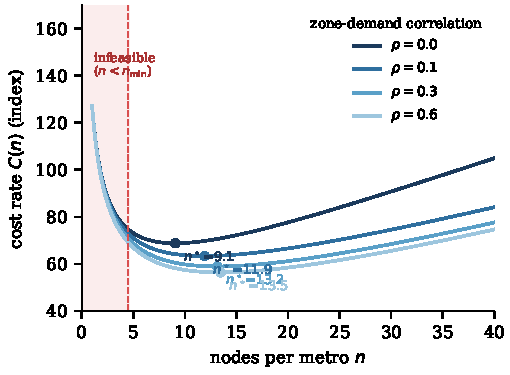
\includegraphics[width=\columnwidth]{costcurve.pdf}
\caption{$^{\mathrm{R5}}$ Illustrative ParaTwin design curve for one metro. Total cost \eqref{eq:cost} is unimodal in $n$; the minimizer $n^\star$ moves right as zone-demand correlation $\rho$ rises, because correlated demand cannot be pooled and decentralization therefore costs less. Revision~4 reported only the $\rho=0$ curve. The network is sized at $\max(n_{\min},n^\star)$, with $n_{\min}$ from Proposition~\ref{prop:radius}; the shaded band marks the SLA-infeasible region. Parameters $(F,a,b)=(1.2,6,120)$ are illustrative and are not Jakarta values.}
\label{fig:cost}
\end{figure}

\subsection{Experiment Portfolio and KPIs}
The launch experiment portfolio is: \textbf{E1} Jakarta node-count sweep $n\in\{5,\dots,40\}$ mixing store nodes and dark MFCs, reporting the curve of Fig.~\ref{fig:cost}; \textbf{E2} assortment depth ladder (150/300/600/1,200 SKUs) against PX1 capture, split-shipment rate, \emph{and order fill rate}$^{\mathrm{R5}}$; \textbf{E3} courier strategy (Grab-only versus dual-carrier versus own-fleet threshold search); \textbf{E4} campaign stress ($10\times$ Hawkes burst during a live event; measures promise-degradation behaviour); \textbf{E5} disruption (hub outage, flood-day travel times $+80\%$, courier surge) with \emph{jointly modelled carrier availability}$^{\mathrm{R5}}$; \textbf{E6} POS-latency and connectivity-outage sensitivity validating conditions (C1)--(C2) of Proposition~\ref{prop:atp}.

$^{\mathrm{R5}}$ Two experiments are added, and they are the only two that can falsify the program rather than tune it:

\textbf{E7 (demand test).} A live promise A/B on brand.com and one marketplace cluster, measuring instant attach rate, conversion lift versus the standard promise, and delivery-fee elasticity, for beauty baskets in Jakarta. E7 does not require the network: it requires a promise and a small number of nodes, and it runs in Phase~0. Revision~4 contained six supply-side experiments and no demand test, so the assumption on which every node economic rests---that Indonesian beauty consumers convert on a 60-minute promise at a rate that clears the break-even volume derived under O-17---was never scheduled to be measured.

\textbf{E8 (incrementality holdout).} A matched-market design over participating versus non-participating consignment stores of similar archetype and catchment, estimating the incremental share of store-node volume against the counterfactual of the walk-in sale \cite{imbens2015,abadie2010}. E8 resolves the contradiction between the partner-benefit and cannibalization framings of Section~\ref{sec:business}.

\begin{table}[t]
\caption{ParaTwin KPI Vector $\mathcal{Y}$ (per scenario, with 95\% CIs). Rows marked $^{\mathrm{R5}}$ are added in this revision.}
\label{tab:kpi}
\centering\footnotesize
\begin{tabular}{@{}p{1.3cm}p{6.3cm}@{}}
\toprule
\textbf{Group} & \textbf{KPIs}\\
\midrule
Promise & $\alpha$-attainment per class; p50/p95 click-to-door; promise-shown rate (\% of zone-hours with PX1 offered); \emph{promise-downgrade rate by cause}$^{\mathrm{R5}}$\\
Economics & Contribution/order (pick, courier, mid-mile, \emph{returns, packaging, commission}$^{\mathrm{R5}}$); routed mid-mile km and batching savings; node break-even attainment; network cost $C(n)$; \emph{incrementality ratio (E8)}$^{\mathrm{R5}}$\\
Inventory & \emph{Order fill rate $\alpha_B$}$^{\mathrm{R5}}$; item fill rate $\beta$; safety stock (units, IDR); substitution and split-shipment rates; expiry/obsolescence risk\\
Operations & Picker utilization; queue-delay probability vs.\ \eqref{eq:staffing}; courier match time; cycle-count variance; \emph{ORE regret vs.\ clairvoyant}$^{\mathrm{R5}}$; \emph{ORE lift vs.\ naive policy (off-policy)}$^{\mathrm{R5}}$\\
Resilience & SLA retention under E5 disruptions; recovery time; re-routing coverage; \emph{Boole-bound vs.\ fitted-quantile radius gap}$^{\mathrm{R5}}$\\
Demand$^{\mathrm{R5}}$ & Instant attach rate; conversion lift vs.\ standard promise; delivery-fee elasticity (E7)\\
\bottomrule
\end{tabular}
\end{table}

\section{Implementation Roadmap}\label{sec:roadmap}

The rollout follows lesson L5 (density before geography) and is twin-gated at every phase. $^{\mathrm{R5}}$ Revision~4 gave acceptance gates to Phases 0--2 and none to Phases 3--4, tested Phase~1 economics against twin agreement rather than against the design target, and contained no condition under which the program stops. All four are corrected.

\textbf{Phase 0 --- Foundations (months 0--4).} Build VIS/DOM and ORE cores; Exagon+ store app with heartbeats; ShipGo+ Grab/GoSend integration; ParaTwin v1 calibrated on MagPie/Tegal history; select the pilot metro (South Jakarta cluster) and run E1--E3 and \textbf{E7}.
\emph{Gate:} twin certification (trace-replay $\le10\%$ deviation, holdout pass, independent policy check); \textbf{and} closure of the eight Phase-0-exit open items O-1 through O-7 and O-23 (Section~\ref{sec:open}), with O-8 and O-25 already closed at Phase~0 start.

\textbf{Phase 1 --- Pilot (months 4--9).} Activate 15--25 consignment store nodes, 2 dark MFCs and 1 flagship MFC in the pilot cluster; brand.com and one marketplace instant program live; run \textbf{E8}.
\emph{Gate:} PX1 $\alpha\ge0.93$ observed \emph{at the order level} (Proposition~\ref{prop:orderfill}); contribution per order $\ge$ the published design-target floor \emph{in absolute terms}, with twin agreement reported separately as a calibration statistic rather than as the acceptance test; store-node pick SLA $\ge90\%$; store-node shrink within the separately stated allowance; E8 incrementality ratio above the published threshold.

\textbf{Phase 2 --- Jakarta scale-out (months 9--18).} Expand to $\max(n_{\min},n^\star)$ nodes for Jabodetabek under the two-stage rule of Section~\ref{sec:arch}-\ref{sec:sizing}; PX2 batched runs and dual-carrier failover live.
\emph{Gate:} network contribution positive; promise-shown rate $\ge80\%$ of metro zone-hours; direct-channel share at or above its stated target (the named mitigation for marketplace program dependence, which Revision~4 listed without a measurable form).

\textbf{Phase 3 --- Multi-metro (months 18--30).} Bandung, Surabaya, Medan, Makassar as regional hubs plus MOSTRANS waves; own-fleet threshold review per cluster; B2B same-day synergy live.
\emph{Gate}$^{\mathrm{R5}}$\emph{:} per-metro re-estimation of $\Lambda$, $\sigma$, $\rho$, $\eta$ and the in-node and travel quantile functions \emph{before} each metro commits, with $n^\star$ and $n_{\min}$ recomputed from local parameters; Jakarta network contribution sustained positive for two consecutive quarters; no metro launches on Jakarta parameters.

\textbf{Phase 4 --- Moat (months 30+).} Anticipatory placement (campaign-aware pre-positioning ahead of live-commerce events); ParaExpress-as-a-service for adjacent halal FMCG brands.
\emph{Gate}$^{\mathrm{R5}}$\emph{:} anticipatory placement demonstrates positive expected value in twin backtest against reactive placement before any capital commitment; third-party service opens only where ParagonCorp volume alone already clears node break-even, so external demand is upside rather than a dependency.

\subsection{$^{\mathrm{R5}}$ Kill Criteria}
Revision~4 stated no condition under which the program should stop, so its gates could only certify that a well-run pilot was well run. The program halts and returns to the marketplace-independent direct-channel scope if any of the following holds:

\begin{enumerate}
\item \textbf{Demand.} E7 shows instant attach rate or conversion lift below the level at which a node reaches its published break-even volume within the Phase-2 horizon, at a delivery fee consumers accept.
\item \textbf{Access.} O-1 resolves negatively at both major marketplaces and direct channels cannot reach the volume threshold in (1).
\item \textbf{Partner supply.} Recruitment conversion is such that the pilot cluster cannot reach $n_{\min}$ from Proposition~\ref{prop:radius} with store nodes plus economically justified MFCs.
\item \textbf{Incrementality.} E8 shows the incremental share of store-node volume below the level at which the program is margin-positive against the walk-in counterfactual.
\item \textbf{Unit economics.} Observed contribution per order is below the design-target floor for two consecutive quarters after the pilot ramp, with no identified and costed remediation.
\end{enumerate}

Each criterion names a measured quantity, a threshold to be published before the measurement is taken, and the experiment that produces it. \OPEN{numeric thresholds for kill criteria 1--5, published before Phase 0 experiments read out}{Head of Platform R\&D + Finance}{Phase 0 start}

\subsection{Risks and Mitigations}
Principal risks and their mitigations: \emph{store data quality} (Proposition~\ref{prop:atp} buffers, effective-latency observation, allocation suspension, locked shelf units); \emph{courier surge and supply} (dual carrier with jointly modelled availability, pre-matching, promise degradation as the real hedge, own-fleet trigger rule); \emph{marketplace program dependence} (direct channels grown against a stated share target and a Phase-2 gate, plus the fallback scope in kill criterion 2); \emph{cannibalization of B2B doors} (measured by E8, not argued); \emph{demand overestimation} (phase gates twin-calibrated with holdout validation, E7 ahead of capital, every node opening reversible because leases are short and store nodes are contractual addenda); \emph{decision-model error} (independent policy check and off-policy scoring, Section~\ref{sec:twin}); \emph{ledger unavailability} (degraded reservation mode, principle P-6).

\section{Open Items Register}\label{sec:open}

Table~\ref{tab:open} registers every fact this specification requires and nobody has yet confirmed. The register exists because a technical document that fills an unknown with a plausible number produces a design that runs and is quietly wrong; a visible hole with an owner and a date stops the decision instead. Ten items block Phase~0. Eight must close before Phase~0 exits---O-1 through O-7 and O-23---because each can invalidate a downstream decision that Phase~1 would otherwise take on a guess. Two must close before Phase~0 \emph{starts}: O-8, because a kill threshold published after the measurement is not a kill threshold, and O-25, because an item with a role but no person has no owner.

\begin{table}[t]
\caption{Open Items Register. \emph{Blocks} names the earliest decision that cannot be taken until the item closes.}
\label{tab:open}
\centering\footnotesize
\begin{tabular}{@{}p{0.5cm}p{4.0cm}p{1.5cm}p{1.0cm}@{}}
\toprule
\textbf{ID} & \textbf{Question} & \textbf{Owner (role)} & \textbf{Blocks}\\
\midrule
O-1 & Written marketplace confirmation that seller-fulfilled instant from brand nodes is permitted, and courier terms & Commercial Lead & Ph.\ 0 exit\\
O-2 & Instant attach rate, conversion lift, delivery-fee elasticity for beauty (E7) & Commercial Lead & Ph.\ 0 exit\\
O-3 & Distinct-SKU basket-size distribution $p_j$ (drives $\beta^\star$, Prop.~\ref{prop:orderfill}) & Data Lead & Ph.\ 0 exit\\
O-4 & Grab/GoSend commercial rate card at projected volume tier & Commercial Lead & Ph.\ 0 exit\\
O-5 & Consignment partner-side P\&L, recruitment pre-test conversion, non-compliance exit path & Consignment Ops & Ph.\ 0 exit\\
O-6 & Heron pick-accuracy and pick-time baselines at Tegal & Warehouse Systems & Ph.\ 0 exit\\
O-7 & Whether channel commission sits inside or outside the 40--55\% gross-margin line & Commercial Lead & Ph.\ 0 exit\\
O-8 & Numeric thresholds for kill criteria 1--5, published before readout & R\&D + Finance & Ph.\ 0 start\\
\midrule
O-9 & Measured packing/overlap efficiency $\eta$ per metro & Data Lead & Ph.\ 1 gate\\
O-10 & Fitted in-node time and effective-speed quantile functions & Data Lead & Ph.\ 1 gate\\
O-11 & Fitted zone-demand equicorrelation $\rho$ by hour and campaign state & Data Lead & Ph.\ 1 gate\\
O-12 & Single-brand basket share by count \emph{and} by revenue ($\epsilon$, $\epsilon_{\mathrm{rev}}$) & Data Lead & Ph.\ 1 gate\\
O-13 & Basket-value distribution and the node-activation contribution floor & Data Lead & Ph.\ 1 gate\\
O-14 & Measured store-node picking capacity under observed walk-in traffic & Consignment Ops & Ph.\ 1 gate\\
O-15 & POS posting-latency and connectivity-uptime distribution across partners & Consignment Ops & Ph.\ 1 gate\\
O-16 & VIS RTO and measured failover time; reservation TTL; composed order-to-pick p99 & Platform Eng & Ph.\ 1 gate\\
O-17 & Missing P\&L lines: returns rate and cost, packaging, carrying cost $h$, employment model, store-node shrink allowance, rent validation, break-even derivation & Finance + Ops & Ph.\ 1 gate\\
O-18 & Joint availability and price correlation of Grab and GoSend & Data Lead & Ph.\ 1 gate\\
O-19 & Minimum back-room footprint holding one week of instant demand (Rev.~4's 20--40\,m$^2$ matches no format) & Platform R\&D & Ph.\ 1 gate\\
O-20 & Proof or counterexample: submodularity of the splittable capacitated coverage value & Platform R\&D & Ph.\ 1 exit\\
O-21 & Own-fleet cost model and the equation behind the threshold & Finance + Commercial & Ph.\ 2 gate\\
O-22 & AOV \emph{distribution} (not mean) by catchment & Data Lead & Ph.\ 1 gate\\
O-23 & Assumed delivery-fee subsidy rate & Commercial Lead & Ph.\ 0 exit\\
O-24 & Regulatory review: BPOM storage and traceability at Tier-2 nodes; halal-chain integrity across consignment partners & Regulatory Affairs & Ph.\ 1 gate\\
O-25 & Named individual owners against every role in this table & Head of Platform R\&D & Ph.\ 0 start\\
\bottomrule
\end{tabular}
\end{table}

\section{Conclusion}

Instant delivery in Indonesia will be won by whoever combines proximity, honesty of promise, and category ownership. This report specifies ParaExpress as ParagonCorp's answer: a two-speed network that preserves the NDC/DC backbone and superimposes a hyperlocal fulfillment tier built first from the consignment estate---a zero-capex coverage endowment formalized by Corollary~\ref{cor:stores}---and completed by cost-engineered dark MFCs sized by Theorem~\ref{thm:nodecount} and Proposition~\ref{prop:radius}.

The mathematics is not decoration. NP-hardness motivates the twin-gated design process; submodularity yields a provably near-optimal rollout order where capacity does not bind, and its failure under capacity (Section~\ref{sec:structural}-\ref{sec:capacitated}) is why the order is recomputed after every activation rather than fixed once; the uniform-matroid result makes weekly assortment refresh exact and cheap; total unimodularity guarantees that real-time routing is exactly solvable inside the sub-100\,ms wave budget; and the square-root laws of pooling and staffing---restated here under demand correlation and wave batching---quantify the density--decentralization trade that sank the first quick-commerce wave.

Revision~5 changes the report in one direction more than any other: it separates what is proved from what is assumed. Two results were being used outside the conditions under which they were proved, and both errors ran the same way, toward a network smaller and cheaper than the promise requires. One quantity that governs the headline promise---order-level availability---had no equation anywhere in Revision~4. The economics rested on a mean where a distribution was needed, and the acceptance gates could be passed by a model that was internally consistent and externally wrong. Correcting these does not weaken the thesis; it raises the capital ask and makes the thesis testable, which is the only form in which it is worth funding.

The competitive thesis inverts the platform playbook: rather than a platform using speed to commoditize brands, the brand uses speed---delivered from within the consumer's own neighborhood---to make the platform the commodity. Whether Indonesian beauty consumers will pay for that speed at the density this design requires is the one thing this report does not know, and experiment E7 exists to find out before the capital does.

\appendices

\section{Design Review Method, Derivations, and Change Register}

This appendix documents how Revision~5's changes were produced. It is included so that a reader can audit the reasoning behind each change rather than accept it on authority, and so that the same review can be re-run against Revision~5.

\subsection{Why a Structured Review, and Why This Structure}

Revision~4 was written by the team that designed ParaExpress, and reviewed by the same team. The empirical software-engineering literature is unusually clear about what beats unstructured review. Fagan's inspection method established that a structured reading with defined roles finds materially more defects than unstructured review \cite{fagan1976}. Porter, Votta and Basili then showed in a replicated controlled experiment that \emph{defect-based scenario reading}---each reviewer works a distinct scenario with its own question list---outperforms both ad hoc and checklist-based review on requirements documents \cite{porter1995}. Basili et al.\ generalized the scenario idea into \emph{perspective-based reading}, in which each reviewer reads the same artifact from one assigned stakeholder viewpoint \cite{basili1996}. The mechanism is coverage: a single reader with a general mandate re-finds the defects their own expertise makes salient, while a set of readers with disjoint mandates covers a wider defect space with the same effort.

The review of Revision~4 therefore assigned six disjoint lenses, each with its own question set:

\begin{enumerate}
\item \textbf{Optimization and mathematics} --- does each theorem prove what the surrounding prose claims; do the stated assumptions hold in the deployment described; is any result used outside its own conditions.
\item \textbf{Fulfillment and inventory operations} --- network tiering, node sizing, forward assortment, base stock, replenishment cadence, staffing, in-node process, returns.
\item \textbf{Platform and systems engineering} --- the new and extended services, interface and event contracts, availability and latency targets, failure modes, consistency, offline paths.
\item \textbf{Unit economics and commercial structure} --- node P\&L, break-even logic, subsidy, partnership terms, cannibalization, capitalization.
\item \textbf{Indonesia execution reality} --- marketplace program dependence, carrier supply, partner incentives and data quality, labour and real estate, regulatory exposure, rollout gates.
\item \textbf{The report as a written argument} --- claims outrunning evidence, benchmark comparability, design targets presented as results, missing sensitivity, notation.
\end{enumerate}

Three procedural rules were applied, each for a documented reason.

\emph{No severity filter at generation time.} The review was instructed to report every improvement found at every severity, and to order rather than suppress. Filtering instructions applied before generation remove findings that the filter's author could not have anticipated; the reader's need for a short list is met instead by severity ordering, a per-finding confidence field, and a ranked ``fix first'' list. This is the same reasoning that motivates full-coverage reading in inspection practice \cite{fagan1976,porter1995}. It is a procedural choice, not an empirical result: no controlled comparison of filtered against unfiltered review is cited here.

\emph{An adversarial pass before publication.} Every finding was then argued against: the strongest case that it was \emph{not} a real problem was constructed, and findings that did not survive were discarded with the reason recorded (Appendix~A-D). This is the premortem discipline \cite{klein2007} applied to the review itself rather than to the plan, and it exists because a multi-lens review generates plausible-but-wrong findings at a rate that would otherwise erode the credibility of the correct ones. Seven of forty-eight candidate findings were discarded at this step, including five where the reviewer's arithmetic or reading was wrong and Revision~4's was right.

\emph{Arithmetic was recomputed, not accepted.} Every numeric claim in Revision~4 that could be checked from the document was recomputed independently, including the cubic root of Theorem~\ref{thm:nodecount}, its $F\to0$ limit, the complexity bound of Theorem~\ref{thm:routing}, the radius-versus-in-node-time arithmetic of Proposition~\ref{prop:radius}, and the picker-throughput consistency of Table~\ref{tab:formats}. All five checked out and are recorded as such.

\subsection{Derivation of Each Correction}

Table~\ref{tab:derivation} maps each material change to the established result it rests on. Nothing in Revision~5 is a novel mathematical contribution: every correction applies a known result that Revision~4 either did not cite or cited in a special case.

\begin{table*}[t]
\caption{Derivation of Revision-5 Corrections}
\label{tab:derivation}
\centering\footnotesize
\begin{tabular}{@{}p{2.5cm}p{5.4cm}p{5.4cm}p{3.0cm}@{}}
\toprule
\textbf{Change} & \textbf{What Revision 4 did} & \textbf{Why it is wrong, and what replaces it} & \textbf{Rests on}\\
\midrule
Prop.~\ref{prop:orderfill} order fill rate (new) & Sized safety stock from an item fill rate $\beta$; promised 95\% measured on the order & An order fails if any basket SKU is missing, so $\alpha_B=G_B(\beta)$; invert to get $\beta^\star=G_B^{-1}(\alpha_B^{\mathrm{tgt}})$. Under positive association the product form is a lower bound, so $\beta^\star$ is conservative & Song \cite{song1998}; Hausman, Lee \& Zhang \cite{hausman1998}; Esary, Proschan \& Walkup \cite{esary1967}\\
Prop.~\ref{prop:radius} service radius (restated) & $R=v(\tau-T_{\mathrm{route}}-t^{\alpha}_{\mathrm{node}})^{+}$ with $v$ a mean speed & Uses $q_\alpha(X+Y)=q_\alpha(X)+\mathbb{E}[Y]$, false for any $Y$ with positive variance; quantiles/VaR are not additive. Replaced by a Boole risk-budget split, distribution-free and dependence-free & Artzner et al.\ \cite{artzner1999}; Embrechts, McNeil \& Straumann \cite{embrechts2002}; Boole's inequality \cite{feller1968}\\
Prop.~\ref{prop:pooling} pooling penalty (restated) & $\sqrt{n}$ safety-stock inflation, independent zones & The design models Hawkes-correlated demand and re-pools via substitution/rebalancing; $\Psi(n,\rho)=\sqrt{n/(1+(n-1)\rho)}$. Eppen's own paper covers the correlated case & Eppen \cite{eppen1979}\\
Thm.~\ref{thm:nodecount} node count (restated) & Unimodal cost with $\sqrt n$ term; single $n^\star$ & Restated on $\Psi(n,\rho)$; $n^\star$ nondecreasing in $\rho$, so Revision~4 biased the node count downward & Follows from Prop.~\ref{prop:pooling}\\
\S\ref{sec:capacitated} capacitated coverage & Cited $(1-1/e)$, proved for $\mu_f=\infty$, in a network with binding throughput caps & Explicit counterexample: capacity creates complementarity, so whole-order coverage is not submodular and greedy loses the bound. Guarantee recovered by a different algorithm & Nemhauser, Wolsey \& Fisher \cite{nemhauser1978} (scope); Chekuri \& Kumar \cite{chekuri2004}; Fleischer et al.\ \cite{fleischer2011}; Ageev \& Sviridenko \cite{ageev2004}\\
Prop.~\ref{prop:staffing} staffing (restated) & Halfin--Whitt on M/M/$c$, with wave-batched release specified elsewhere & Wave release makes arrivals compound Poisson; index of dispersion $1+\lambda_f\Delta$ inflates the safety term by its square root, making $\Delta$ a two-sided decision & Halfin \& Whitt \cite{halfin1981}; Whitt \cite{whitt1993,whitt2004}; Chaudhry \& Templeton \cite{chaudhry1983}\\
Prop.~\ref{prop:atp} ATP safety (restated) & Single-partition invariant with fixed 5-min posting latency & Adds effective latency from liveness heartbeats, allocation suspension, and a cross-partition commit rule for rebalancing and split shipment & Herlihy \& Wing \cite{herlihy1990}; Gray \& Reuter \cite{gray1993}; Garcia-Molina \& Salem \cite{garciamolina1987}; Gilbert \& Lynch \cite{gilbert2002}\\
\S\ref{sec:commit} commitment policy (new) & ``Re-solved every few seconds'' with per-wave optimality claimed & States the commitment rule, reframes the router as online, and measures regret against clairvoyant instead of claiming an unproven bound & Klapp et al.\ \cite{klapp2018}; Ulmer et al.\ \cite{ulmer2021}; Lan et al.\ \cite{lan2024}\\
Thm.~\ref{thm:assortment}(iv) basket bound & Degradation factor $(1-\epsilon)$ with $\epsilon$ a basket \emph{count} share & The objective measures revenue, so the bound must be on revenue share $\epsilon_{\mathrm{rev}}$; cross-brand baskets are plausibly larger than average & Sviridenko \cite{sviridenko2004}; Kellerer, Pferschy \& Pisinger \cite{kellerer2004}\\
Twin policy check (new) & Shared decision code presented as pure benefit & Shared code removes drift and removes independent verification of the decision model; adds an off-policy scored held-out policy & Sargent \cite{sargent2013}; Li et al.\ \cite{li2011}\\
E8 incrementality (new) & Cannibalization listed as a risk and the same mechanism sold as a benefit & Makes incrementality a measured treatment effect with a matched-market design & Imbens \& Rubin \cite{imbens2015}; Abadie, Diamond \& Hainmueller \cite{abadie2010}\\
Kill criteria (new) & Gates tested execution quality only; no stop condition & A design with no falsifying observation cannot be tested by its own gates; adds five measurable stop conditions with pre-published thresholds & Popper \cite{popper1959}; Klein \cite{klein2007}; Flyvbjerg \cite{flyvbjerg2006}\\
Appendix~B sensitivity (new) & One illustrative curve, parameters fixed & Design rests on parameters with no stated ranges; adds ranked variance contribution over the inputs of Thm.~\ref{thm:nodecount} and Prop.~\ref{prop:radius} & Saltelli et al.\ \cite{saltelli2008}\\
\bottomrule
\end{tabular}
\end{table*}

\subsection{Findings Implemented Without New Mathematics}

Fourteen findings required specification rather than derivation and are implemented in the body: per-cell provenance marks in Table~\ref{tab:bench}; the target-versus-observed framing of the capability comparison; the two-stage sizing procedure of Section~\ref{sec:arch}-\ref{sec:sizing}; the contribution floor in Corollary~\ref{cor:stores}; the returns operating model (Section~\ref{sec:mfc}-\ref{sec:returns}); intra-day lateral replenishment (Section~\ref{sec:mfc}-\ref{sec:lateral}); removal of the unsupported store-node throughput range; a separate store-node shrink allowance; the ADR per-input staleness contract; the composed-path latency requirement; the VIS degraded reservation mode and RTO; target-aware decision-log replay and a stated reservation TTL; per-metro gates for Phases 3 and 4; and the direct-channel share target that converts a named mitigation into a measurable one.

\subsection{Findings Deferred to Open Items}

Fourteen findings named a quantity the design depends on and nobody has measured. These are not resolved by argument, and writing a plausible value in their place would produce a specification that runs and is quietly wrong. Each is marked inline at the point of use and registered in Table~\ref{tab:open} with an owner and the decision it blocks. The fourteen findings expand into twenty-five register rows, because several of them name more than one unmeasured quantity: the node-economics finding alone contributes seven. Ten rows block Phase~0.

\subsection{Findings Examined and Rejected}

Seven candidate findings did not survive the adversarial pass. They are recorded so that they are not raised again.

\begin{enumerate}
\item \emph{``Theorem~\ref{thm:hardness}'s Set Cover reduction is invalid.''} Checked. One zone per element, one candidate node per set with zero-cost coverage, uniform fixed cost $\varepsilon$, and $M\gg|\mathcal{S}|\varepsilon$ jointly force any optimal solution to cover all zones and then minimize node count. The reduction is standard and correct.
\item \emph{``The worked numbers of Remark~\ref{rem:numval} do not check.''} They do. $2.4x^3+6x^2-120=0$ has its unique positive root at $x\approx3.012$, giving $n^\star\approx9.07$ and $C(n^\star)\approx68.8$; the $F\to0$ limit $b/a=20$ is also correct.
\item \emph{``Table~\ref{tab:formats} node throughput contradicts the stated picker rate.''} It does not: at 10 orders per picker-hour, 2--6 pickers map onto the stated 20--60 orders/hour for a dark MFC and 6--15 pickers onto 60--150 for a flagship. The store-node row is a separate and real problem, recorded as O-14.
\item \emph{``The claim that 3 minutes of in-node time buys 1\,km of radius at 20\,km/h is wrong.''} It is right, and the quadratic node-count consequence follows correctly from $n_{\min}\propto R^{-2}$.
\item \emph{``Theorem~\ref{thm:routing}'s $O(|O|^2|\mathcal{F}|)$ bound is overstated.''} It is not. Successive shortest paths over a bipartite graph with $O(|O||\mathcal{F}|)$ arcs, one unit augmentation per order, each a Dijkstra pass with Johnson potentials, gives the stated bound up to logarithmic factors.
\item \emph{``The cubic of Theorem~\ref{thm:nodecount} is misderived.''} Verified by differentiation and substitution.
\item \emph{``Propositions~\ref{prop:pooling} and~\ref{prop:staffing} contradict each other by making decentralization simultaneously costly and cheap.''} They do not. Both penalize splitting---one in inventory, one in labour---and both counterbalance the coverage pressure of Proposition~\ref{prop:radius}. The report's framing is consistent.
\end{enumerate}

\subsection{What This Review Did Not Cover}

Three areas were outside the review's scope and remain unexamined: legal and regulatory exposure (halal certification handling at fulfillment nodes, cosmetics-specific BPOM requirements for storage and traceability, employment classification risk); information security beyond the transport and access controls stated in Section~\ref{sec:solution}; and the accuracy of the third-party market figures in Section~\ref{sec:bench} beyond marking their provenance. Each should carry its own review before Phase~1 commits; the regulatory gap is registered as O-24 and the other two are named here without a register row, because neither yet names a specific unknown quantity.

\section{Sensitivity Analysis}

Revision~4 reported one design curve at one parameter set. Because $n^\star$ and $n_{\min}$ jointly set the capital ask, the recruitment target and the phase plan, the design requires a stated uncertainty on both. Revision~5 specifies the analysis rather than reporting a result, because the input ranges are open items (O-9 through O-13).

The required output is a ranked variance-contribution analysis \cite{saltelli2008} over the inputs of Theorem~\ref{thm:nodecount} ($F$, $h$, $z_{\beta^\star}$, $\sigma$, $\rho$, $\Lambda$, $c_d$, $k$, $A$) and Proposition~\ref{prop:radius} ($\tau$, $T_{\mathrm{route}}$, the in-node and speed quantile functions, $\eta$), with each input's range sourced and cited, and with $n^\star$ and $n_{\min}$ reported as intervals rather than point values. Three interactions are known in advance to be material and must be reported explicitly: $\rho$ against $\sigma$ (both act on the pooling term, in opposite directions); $\beta^\star$ against the basket-size distribution (Proposition~\ref{prop:orderfill} makes safety stock a function of basket composition, not only of demand variability); and in-node time against $\eta$ (both enter $n_{\min}$, one linearly through the radius and one directly, so a metro with poor packing efficiency and slow picking compounds).

The illustrative sweeps already computed give the order of magnitude at stake. Holding all else at the Revision~4 values, $n^\star$ moves from 9.1 to 13.6 as $\rho$ moves from 0 to 0.9; and under the illustrative time and speed distributions of Section~\ref{sec:structural}, $n_{\min}$ changes by a factor of 3.5 between Revision~4's radius formula and Proposition~\ref{prop:radius}. Neither range was visible in Revision~4. The pooling range moves the deployed node count directly; the radius range does not bind on the illustrative parameters but determines whether $n_{\min}$ or $n^\star$ is the binding constraint, which is not knowable until O-9 and O-10 close.


\begin{thebibliography}{99}
\footnotesize

\bibitem{chandra2026} R. Chandra \emph{et al.}, ``Regionalize and scale: Amazon's fulfillment network design for faster and cheaper delivery,'' \emph{INFORMS J. Appl. Analytics}, vol.~56, no.~1, pp.~23--41, Jan.~2026.
\bibitem{amazonscience} Amazon Science, ``Sizing down to scale up: How Amazon reworked its fulfillment network to meet customer demand,'' 2023. [Online].
\bibitem{supplychaindive2023} Supply Chain Dive, ``Amazon shifts to regional fulfillment model,'' 2023. [Online].
\bibitem{costar2024} CoStar News, ``Amazon to double number of same-day delivery centers after initial success,'' 2024. [Online].
\bibitem{palmer2024} A. Palmer, ``Amazon says 60\% of Prime orders are arriving same day or next day,'' CNBC, Apr.~29, 2024. [Online].
\bibitem{redstag} Red Stag Fulfillment, ``How many Amazon warehouses are there?'' 2025. [Online].
\bibitem{amazon2023robots} Amazon, ``Amazon announces new fulfillment center robots, Sequoia and Digit,'' About Amazon, Oct.~2023. [Online].
\bibitem{techcrunch2025} TechCrunch, ``Amazon deploys its 1 millionth robot, releases generative AI model,'' Jul.~1, 2025. [Online].
\bibitem{spiegel2013} J.~R. Spiegel, M.~T. McKenna, G.~S. Lakshman, and P.~G. Nordstrom, ``Method and system for anticipatory package shipping,'' U.S. Patent 8\,615\,473 B2, Dec.~24, 2013.
\bibitem{wirechina2024} The Wire China, ``Can Alibaba deliver?'' Jan.~28, 2024. [Online].
\bibitem{scmp2023} South China Morning Post, ``Alibaba logistics unit Cainiao unveils express service to improve e-commerce efficiency,'' 2023. [Online].
\bibitem{vangaalen2022} E. van Gaalen, ``Hit and miss---The ultimate guide to Alibaba's Hema (Freshippo) store formats, Part 1,'' ChinaTalk, 2022. [Online].
\bibitem{statista2024} Statista, ``JD Logistics: Number of warehouses 2024,'' 2024. [Online].
\bibitem{wang2025} X. Wang \emph{et al.}, ``JD.com improves fulfillment efficiency with data-driven integrated assortment planning and inventory allocation,'' \emph{INFORMS J. Appl. Analytics}, 2025.
\bibitem{goodwater2021} Goodwater Capital, ``Understanding Coupang: Setting a new bar for e-commerce (S-1/IPO teardown),'' 2021. [Online].
\bibitem{coupang2025} Coupang, Inc., ``Coupang: A global leader in technology innovation,'' 2025. [Online].
\bibitem{suitefleet2025} SuiteFleet, ``The complete guide to quick-commerce operations,'' 2025. [Online].
\bibitem{browne2024} R. Browne, ``Grocery startup Getir to exit US, Europe and UK, refocus on Turkey,'' CNBC, Apr.~29, 2024. [Online].
\bibitem{sifted2024} Sifted (Financial Times), ``What's left of Europe's speedy grocery sector?'' 2024. [Online].
\bibitem{mohan2025} M. Mohan, ``State of Indian quick commerce market 2025---Blinkit, Zepto, Big Basket, Swiggy and Zomato,'' May~2025. [Online].
\bibitem{storyboard2025} Storyboard18, ``Dark stores explained: How Blinkit, Zepto are building dense networks for quick commerce growth,'' 2025. [Online].
\bibitem{scd2025} Supply Chain Dive, ``Walmart expands same-day delivery reach,'' 2025. [Online].
\bibitem{target2023} Target Corp., ``We're expanding next-day delivery capabilities (sortation centers fact sheet),'' 2023. [Online].
\bibitem{magpieiq2026} Magpie IQ, ``Shopee market share in Indonesia: Live platform data,'' 2026. [Online].
\bibitem{databoks2024} Databoks/Katadata (Compas data), ``Shopee dominates Indonesia's beauty product e-commerce market,'' 2024. [Online].
\bibitem{spx2025} SPX Express Indonesia, ``Layanan pengiriman SPX Express,'' 2025. [Online].
\bibitem{mordor2024} Mordor Intelligence, ``Indonesia e-commerce market trends, growth \& share (to 2031),'' 2024. [Online].
\bibitem{nikkei2023} Nikkei Asia, ``China-owned TikTok to invest \$1.5bn in Tokopedia, take 75\% stake,'' Dec.~2023. [Online].
\bibitem{moca2026} MOCA Technology, ``TikTok Shop Indonesia: From ban to \$13.8B GMV,'' 2026. [Online].
\bibitem{theken2023} The Ken, ``Where quick-commerce startups fail, Indonesia's Astro sees ways to make a fast buck,'' 2023. [Online].
\bibitem{gpca2024} Global Private Capital Association and AC Ventures, ``Astro Technologies Indonesia (case study),'' 2024. [Online].
\bibitem{grab2025} Grab, ``GrabExpress Instant \& Same Day package \& document delivery (merchant API),'' 2025. [Online].
\bibitem{gojek2024} Gojek/GoTo, ``Integrasi API GoSend,'' 2024. [Online].
\bibitem{ssi2022} Supply Chain Indonesia, ``Platform digital Mostrans optimalkan layanan distribusi dan logistik,'' 2022. [Online].
\bibitem{kalbe2019} Kalbe Farma, ``Kalbe Group launches digital transportation platform first in Indonesia for the health industry,'' 2019. [Online].
\bibitem{rm2026} ResearchAndMarkets, ``Indonesia quick commerce report 2026: Market to reach \$1.83 billion by 2029,'' GlobeNewswire, Apr.~2026. [Online].

\bibitem{daskin2013} M.~S. Daskin, \emph{Network and Discrete Location: Models, Algorithms, and Applications}, 2nd~ed. Hoboken, NJ: Wiley, 2013.
\bibitem{melo2009} M.~T. Melo, S. Nickel, and F. Saldanha-da-Gama, ``Facility location and supply chain management---A review,'' \emph{Eur. J. Oper. Res.}, vol.~196, no.~2, pp.~401--412, 2009.
\bibitem{church1974} R. Church and C.~S. ReVelle, ``The maximal covering location problem,'' \emph{Papers Regional Sci. Assoc.}, vol.~32, pp.~101--118, 1974.
\bibitem{garey1979} M.~R. Garey and D.~S. Johnson, \emph{Computers and Intractability: A Guide to the Theory of NP-Completeness}. San Francisco, CA: Freeman, 1979.
\bibitem{nemhauser1978} G.~L. Nemhauser, L.~A. Wolsey, and M.~L. Fisher, ``An analysis of approximations for maximizing submodular set functions---I,'' \emph{Math. Program.}, vol.~14, no.~1, pp.~265--294, 1978.
\bibitem{cornuejols1977} G. Cornuejols, M.~L. Fisher, and G.~L. Nemhauser, ``Location of bank accounts to optimize float: An analytic study of exact and approximate algorithms,'' \emph{Manage. Sci.}, vol.~23, no.~8, pp.~789--810, 1977.
\bibitem{feige1998} U. Feige, ``A threshold of $\ln n$ for approximating set cover,'' \emph{J. ACM}, vol.~45, no.~4, pp.~634--652, 1998.
\bibitem{fleischer2011} L. Fleischer, M.~X. Goemans, V.~S. Mirrokni, and M. Sviridenko, ``Tight approximation algorithms for maximum separable assignment problems,'' \emph{Math. Oper. Res.}, vol.~36, no.~3, pp.~416--431, 2011.
\bibitem{chekuri2004} C. Chekuri and A. Kumar, ``Maximum coverage problem with group budget constraints and applications,'' in \emph{APPROX/RANDOM 2004}, LNCS 3122, pp.~72--83.
\bibitem{ageev2004} A.~A. Ageev and M. Sviridenko, ``Pipage rounding: A new method of constructing algorithms with proven performance guarantee,'' \emph{J. Comb. Optim.}, vol.~8, no.~3, pp.~307--328, 2004.
\bibitem{eppen1979} G.~D. Eppen, ``Effects of centralization on expected costs in a multi-location newsboy problem,'' \emph{Manage. Sci.}, vol.~25, no.~5, pp.~498--501, 1979.
\bibitem{daganzo1984} C.~F. Daganzo, ``The distance traveled to visit $N$ points with a maximum of $C$ stops per vehicle: An analytic model and an application,'' \emph{Transp. Sci.}, vol.~18, no.~4, pp.~331--350, 1984.
\bibitem{song1998} J.-S. Song, ``On the order fill rate in a multi-item, base-stock inventory system,'' \emph{Oper. Res.}, vol.~46, no.~6, pp.~831--845, 1998.
\bibitem{hausman1998} W.~H. Hausman, H.~L. Lee, and A.~X. Zhang, ``Joint demand fulfillment probability in a multi-item inventory system with independent order-up-to policies,'' \emph{Eur. J. Oper. Res.}, vol.~109, no.~3, pp.~646--659, 1998.
\bibitem{esary1967} J.~D. Esary, F. Proschan, and D.~W. Walkup, ``Association of random variables, with applications,'' \emph{Ann. Math. Statist.}, vol.~38, no.~5, pp.~1466--1474, 1967.
\bibitem{artzner1999} P. Artzner, F. Delbaen, J.-M. Eber, and D. Heath, ``Coherent measures of risk,'' \emph{Math. Finance}, vol.~9, no.~3, pp.~203--228, 1999.
\bibitem{embrechts2002} P. Embrechts, A. McNeil, and D. Straumann, ``Correlation and dependence in risk management: Properties and pitfalls,'' in \emph{Risk Management: Value at Risk and Beyond}. Cambridge, U.K.: Cambridge Univ. Press, 2002, pp.~176--223.
\bibitem{feller1968} W. Feller, \emph{An Introduction to Probability Theory and Its Applications}, vol.~I, 3rd~ed. New York: Wiley, 1968.
\bibitem{kellerer2004} H. Kellerer, U. Pferschy, and D. Pisinger, \emph{Knapsack Problems}. Berlin, Germany: Springer, 2004.
\bibitem{sviridenko2004} M. Sviridenko, ``A note on maximizing a submodular set function subject to a knapsack constraint,'' \emph{Oper. Res. Lett.}, vol.~32, no.~1, pp.~41--43, 2004.
\bibitem{ahuja1993} R.~K. Ahuja, T.~L. Magnanti, and J.~B. Orlin, \emph{Network Flows: Theory, Algorithms, and Applications}. Englewood Cliffs, NJ: Prentice-Hall, 1993.
\bibitem{halfin1981} S. Halfin and W. Whitt, ``Heavy-traffic limits for queues with many exponential servers,'' \emph{Oper. Res.}, vol.~29, no.~3, pp.~567--588, 1981.
\bibitem{whitt1993} W. Whitt, ``Approximations for the GI/G/m queue,'' \emph{Prod. Oper. Manage.}, vol.~2, no.~2, pp.~114--161, 1993.
\bibitem{whitt2004} W. Whitt, ``A diffusion approximation for the G/GI/n/m queue,'' \emph{Oper. Res.}, vol.~52, no.~6, pp.~922--941, 2004.
\bibitem{chaudhry1983} M.~L. Chaudhry and J.~G.~C. Templeton, \emph{A First Course in Bulk Queues}. New York: Wiley, 1983.
\bibitem{toth2014} P. Toth and D. Vigo, Eds., \emph{Vehicle Routing: Problems, Methods, and Applications}, 2nd~ed. Philadelphia, PA: SIAM, 2014.
\bibitem{clarke1964} G. Clarke and J.~W. Wright, ``Scheduling of vehicles from a central depot to a number of delivery points,'' \emph{Oper. Res.}, vol.~12, no.~4, pp.~568--581, 1964.
\bibitem{ropke2006} S. Ropke and D. Pisinger, ``An adaptive large neighborhood search heuristic for the pickup and delivery problem with time windows,'' \emph{Transp. Sci.}, vol.~40, no.~4, pp.~455--472, 2006.
\bibitem{vidal2022} T. Vidal, ``Hybrid genetic search for the CVRP: Open-source implementation and SWAP* neighborhood,'' \emph{Comput. Oper. Res.}, vol.~140, art.~105643, 2022.
\bibitem{wouda2024} N.~A. Wouda, L. Lan, and W. Kool, ``PyVRP: A high-performance VRP solver package,'' \emph{INFORMS J. Comput.}, vol.~36, no.~4, pp.~943--955, 2024.
\bibitem{helsgaun2017} K. Helsgaun, ``An extension of the Lin--Kernighan--Helsgaun TSP solver for constrained traveling salesman and vehicle routing problems,'' Roskilde Univ., Roskilde, Denmark, Tech. Rep., 2017.
\bibitem{voigt2025} S. Voigt, ``A review and ranking of operators in adaptive large neighborhood search for vehicle routing problems,'' \emph{Eur. J. Oper. Res.}, vol.~322, no.~2, pp.~357--375, 2025.
\bibitem{christiaens2020} J. Christiaens and G. Vanden Berghe, ``Slack induction by string removals for vehicle routing problems,'' \emph{Transp. Sci.}, vol.~54, no.~2, pp.~417--433, 2020.
\bibitem{kool2019} W. Kool, H. van Hoof, and M. Welling, ``Attention, learn to solve routing problems!'' in \emph{Proc. ICLR}, 2019.
\bibitem{kwon2020} Y.-D. Kwon \emph{et al.}, ``POMO: Policy optimization with multiple optima for reinforcement learning,'' in \emph{Adv. NeurIPS}, vol.~33, 2020, pp.~21188--21198.
\bibitem{luo2023} F. Luo, X. Lin, F. Liu, Q. Zhang, and Z. Wang, ``Neural combinatorial optimization with heavy decoder: Toward large scale generalization,'' in \emph{Adv. NeurIPS}, vol.~36, 2023.
\bibitem{ye2024} H. Ye \emph{et al.}, ``GLOP: Learning global partition and local construction for solving large-scale routing problems in real-time,'' in \emph{Proc. AAAI}, vol.~38, no.~18, 2024, pp.~20284--20292.
\bibitem{lan2024} L. Lan, J.~M.~H. van Doorn, N.~A. Wouda, A. Rijal, and S. Bhulai, ``An iterative sample scenario approach for the dynamic dispatch waves problem,'' \emph{Transp. Sci.}, vol.~58, no.~4, pp.~726--740, 2024.
\bibitem{klapp2018} M.~A. Klapp, A.~L. Erera, and A. Toriello, ``The dynamic dispatch waves problem for same-day delivery,'' \emph{Eur. J. Oper. Res.}, vol.~271, no.~2, pp.~519--534, 2018.
\bibitem{ulmer2021} M.~W. Ulmer, B.~W. Thomas, A.~M. Campbell, and N. Woyak, ``The restaurant meal delivery problem: Dynamic pickup and delivery with deadlines and random ready times,'' \emph{Transp. Sci.}, vol.~55, no.~1, pp.~75--100, 2021.
\bibitem{ortools2025} V. Furnon and L. Perron, \emph{OR-Tools Routing Library}, v9.12. Google, 2025. [Online].

\bibitem{herlihy1990} M.~P. Herlihy and J.~M. Wing, ``Linearizability: A correctness condition for concurrent objects,'' \emph{ACM Trans. Program. Lang. Syst.}, vol.~12, no.~3, pp.~463--492, 1990.
\bibitem{gray1993} J. Gray and A. Reuter, \emph{Transaction Processing: Concepts and Techniques}. San Mateo, CA: Morgan Kaufmann, 1993.
\bibitem{garciamolina1987} H. Garcia-Molina and K. Salem, ``Sagas,'' in \emph{Proc. ACM SIGMOD}, 1987, pp.~249--259.
\bibitem{gilbert2002} S. Gilbert and N. Lynch, ``Brewer's conjecture and the feasibility of consistent, available, partition-tolerant web services,'' \emph{ACM SIGACT News}, vol.~33, no.~2, pp.~51--59, 2002.

\bibitem{ivanov2021} D. Ivanov and A. Dolgui, ``A digital supply chain twin for managing the disruption risks and resilience in the era of Industry 4.0,'' \emph{Prod. Plann. Control}, vol.~32, no.~9, pp.~775--788, 2021.
\bibitem{le2024} T.~V. Le and R. Fan, ``Digital twins for supply chain and logistics systems: Literature review, conceptual framework, research potential, and practical challenges,'' \emph{Comput. Ind. Eng.}, vol.~187, art.~109768, 2024.
\bibitem{snoeck2022} A. Snoeck and M. Winkenbach, ``A discrete simulation-based optimization algorithm for the design of highly responsive last-mile distribution networks,'' \emph{Transp. Sci.}, vol.~56, no.~1, pp.~201--222, 2022.
\bibitem{law2015} A.~M. Law, \emph{Simulation Modeling and Analysis}, 5th~ed. New York: McGraw-Hill, 2015.
\bibitem{sargent2013} R.~G. Sargent, ``Verification and validation of simulation models,'' \emph{J. Simulation}, vol.~7, no.~1, pp.~12--24, 2013.
\bibitem{li2011} L. Li, W. Chu, J. Langford, and X. Wang, ``Unbiased offline evaluation of contextual-bandit-based news article recommendation algorithms,'' in \emph{Proc. WSDM}, 2011, pp.~297--306.
\bibitem{saltelli2008} A. Saltelli \emph{et al.}, \emph{Global Sensitivity Analysis: The Primer}. Chichester, U.K.: Wiley, 2008.
\bibitem{imbens2015} G.~W. Imbens and D.~B. Rubin, \emph{Causal Inference for Statistics, Social, and Biomedical Sciences}. Cambridge, U.K.: Cambridge Univ. Press, 2015.
\bibitem{abadie2010} A. Abadie, A. Diamond, and J. Hainmueller, ``Synthetic control methods for comparative case studies,'' \emph{J. Amer. Statist. Assoc.}, vol.~105, no.~490, pp.~493--505, 2010.

\bibitem{fagan1976} M.~E. Fagan, ``Design and code inspections to reduce errors in program development,'' \emph{IBM Syst. J.}, vol.~15, no.~3, pp.~182--211, 1976.
\bibitem{porter1995} A.~A. Porter, L.~G. Votta, and V.~R. Basili, ``Comparing detection methods for software requirements inspections: A replicated experiment,'' \emph{IEEE Trans. Softw. Eng.}, vol.~21, no.~6, pp.~563--575, 1995.
\bibitem{basili1996} V.~R. Basili \emph{et al.}, ``The empirical investigation of perspective-based reading,'' \emph{Empirical Softw. Eng.}, vol.~1, no.~2, pp.~133--164, 1996.
\bibitem{klein2007} G. Klein, ``Performing a project premortem,'' \emph{Harvard Bus. Rev.}, vol.~85, no.~9, pp.~18--19, 2007.
\bibitem{flyvbjerg2006} B. Flyvbjerg, ``From Nobel Prize to project management: Getting risks right,'' \emph{Project Manage. J.}, vol.~37, no.~3, pp.~5--15, 2006.
\bibitem{popper1959} K. Popper, \emph{The Logic of Scientific Discovery}. London, U.K.: Hutchinson, 1959.

\end{thebibliography}

\end{document}
